% $Id$
%%%%%%%%%%%%%%%%%%%%%%%%%%%%%%%%%%%%%%%%%%%%%%%%%%%%%%%%%%%%%%%%%%%%%%%%%%
%
% C H A P T E R   T H R E E :  P R I M E S
%
%%%%%%%%%%%%%%%%%%%%%%%%%%%%%%%%%%%%%%%%%%%%%%%%%%%%%%%%%%%%%%%%%%%%%%%%%%

\newpage
% \hypertarget{Kapitel_2}{}
\chapter{Prime Numbers}
\label{Label_Kapitel_Primes}
(Bernhard Esslinger, May 1999; Updates Nov. 2000, Dec. 2001, June 2003, May 2005, March 2006, June 2007, January 2010)

\begin{center}
\fbox{\parbox{15cm}{
    \emph{Albert Einstein\footnotemark:}\\
    Progress requires exchange of knowledge.
}}
\end{center}
\addtocounter{footnote}{0}\footnotetext{%
  Albert Einstein, German physicist and Nobel Prize winner, 
  Mar 14, 1879 $-$ Apr 14, 1955.
}

% --------------------------------------------------------------------------
\section{What are prime numbers?}
\index{Prime number} \index{Number!prime}
Prime numbers are whole, positive numbers greater than or equal to $2$ that can
only be divided by 1 and themselves. All other natural numbers greater than or
equal to $2$ can be formed by multiplying prime numbers.

The {\em natural} \index{Number!natural} numbers $\mathbb{N}=\{1, 2, 3, 4,\cdots \}$ thus comprise 
\begin{itemize}
   \item the number $1$ (the unit value)
   \item the primes and
   \item the composite numbers.
\end{itemize}

Prime numbers are particularly important for 3 reasons:
\begin{itemize}
  \item In number theory, they are considered to be the basic components of
natural numbers, upon which numerous brilliant mathematical ideas are based.
  \item They are of extreme practical importance in modern
\index{Cryptography!modern} cryptography (public key \index{Cryptography!public key} cryptography). The most common public key procedure, invented at the end of
the 1970's, is \index{RSA} RSA encryption. Only using (large) prime numbers for
particular parameters can you guarantee that an algorithm is secure, both for
the RSA procedure and for even more modern procedures (digital
\index{Signature!digital} signature, elliptic curves).
  \item The search for the largest known prime numbers does not have any
practical usage known to date, but requires the best computers, is an excellent
benchmark (possibility for determining the performance\index{Performance} of computers) and leads
to new calculation methods on many computers \\
(see also: \url{http://www.mersenne.org/prime.htm}).
\end{itemize}
Many people have been fascinated by prime numbers over the past two millennia.
Ambition to make new discoveries about prime numbers has often resulted in
brilliant ideas and conclusions. The following section provides an easily
comprehensible introduction to the basics of prime numbers. We will also
explain what is known about the distribution (density, number of prime numbers
in particular intervals) of prime numbers and how prime number tests work.


% --------------------------------------------------------------------------
\section{Prime numbers in mathematics}\label{primesinmath}

Every whole number has a factor. The number 1 only has one factor,
itself, whereas the number $12$ has the six factors $1, 2, 3, 4,
6, 12$. Many numbers can only be divided by themselves and by $1$.
With respect to multiplication, these are the ``atoms'' in the
area of numbers. Such numbers are called prime numbers.

In mathematics, a slightly different (but equivalent) definition is used.

\begin{definition}\label{def-pz-prime}
A whole number $p \in {\bf N}$ is called prime \index{Number!prime} if
$p > 1$ and $p$ only possesses the trivial factors $\pm 1$ and $\pm p$.
\end{definition}


By definition, the number $1$ is not a prime number. In the following sections,
$p$ will always denote a prime number.

The sequence of prime numbers starts with $$ 2,~ 3,~ 5,~ 7, ~ 11, ~ 13, ~
17, ~ 19, ~ 23, ~ 29, ~ 31, ~ 37, ~ 41, ~ 43, ~ 47, ~ 53, ~ 59, ~ 61,
~ 67, ~ 71, ~ 73, ~ 79, ~ 83, ~ 89, ~ 97, \cdots . $$
The first 100 numbers include precisely 25 prime numbers. After this,
the percentage of primes constantly decreases. Prime numbers can be
factorized in a uniquely {\em trivial} way: 
$$5 = 1 \cdot 5,\quad  17 = 1 \cdot 17, \quad 1,013 = 1 \cdot 1,013,  \quad
1,296,409 = 1 \cdot 1,296,409.$$
All numbers that have $2$ or more factors not equal 1 are called 
\index{Number!composite} {\em composite} numbers. 
These include $$ 4 = 2 \cdot 2, \quad 6 = 2\cdot 3 $$ as well
as numbers that {\em look like primes}, but are in fact composite:
$$ 91 = 7 \cdot 13, \quad 161=7 \cdot 23, \quad 767 =13 \cdot 59. $$

\begin{theorem}\label{thm-pz-sqr}
Each whole number $m$ greater than $1$ possesses a lowest factor greater than
$1$. This is a prime number $p$. Unless $m$ is a prime number itself, then: $p$
is less than or equal to the square root of $m$.
\end{theorem}

All whole numbers greater than $1$ can be expressed as a product of prime
numbers --- in a unique way. This is the claim of the \textbf{1st fundamental theorem of
number theory} (= fundamental theorem of arithmetic = fundamental building block
of all positive integers).\index{Number theory!fundamental theorem}

\begin{theorem}\label{thm-pz-prod}
Each element $n$ of the natural numbers greater than $1$ can be written as the
product $n = p_1 \cdot p_2 \dots p_m$ of prime numbers. If two such
factorizations $$n =  p_1 \cdot p_2 \cdot \cdots \cdot p_m = p'_1 \cdot p'_2 \cdots
p'_{m'}$$ are given, then they can be reordered such that $\;m = m'\;$ and for
all $i$:  $\;p_i = p'_i$. \\
($p_1, p_2, \dots, p_m$ are called the prime factors of n).
\end{theorem}

In other words: each natural number other than $1$ can be written as a product
of prime numbers in precisely one way, if we ignore the order of the factors.
The factors are therefore unique (the {\em expression as a product of factors}
is unique)! For example, $$ 60 = 2 \cdot 2 \cdot 3 \cdot 5 = 2^2\cdot 3^1 \cdot
5^1. $$
And this --- other than changing the order of the factors --- is the only way in
which the number $60$ can be factorized. If you allow numbers other than primes
as factors, there are several ways of factorizing integers and the \textbf{uniqueness} \hypertarget{uniqueness}{} is
lost: $$ 60 = 1 \cdot 60 = 2 \cdot 30 = 4 \cdot 15 = 5 \cdot 12 =6 \cdot 10 = 2
\cdot 3 \cdot 10 = 2 \cdot 5 \cdot 6 = 3 \cdot 4 \cdot 5 = \cdots . $$

The following section is aimed more at those familiar with mathematical logic:
The 1st fundamental theorem only appears to be obvious \label{remFundTheoOfArithm}. We can construct
numerous other sets of numbers (i.e. other than positive whole numbers greater
than 1), for which numbers in the set cannot be expressed uniquely as a product
of the prime numbers of the set: In the set $M = \{1, 5, 10, 15, 20, \cdots\}$
there is no equivalent to the fundamental theorem under multiplication. The
first five prime numbers of this sequence are $5, 10, 15, 20, 30$ (note: $10$ is
prime, because $5$ is not a factor of $10$ in this set --- the result is not an
element of the given basic set $M$). Because the following applies in $M$: $$
100 = 5 \cdot 20 = 10 \cdot 10 $$ and $5, 10, 20$ are all prime numbers in this
set, the expression as a product of prime factors is not unique here.

% --------------------------------------------------------------------------
\section{How many prime numbers are there?}

For the natural numbers, the primes can be compared to elements in chemistry or
the elementary particles in physics (see \cite[p. 22]{pr:Blum1999}).

Although there are only $92$ natural chemical elements, the number of prime
numbers is unlimited. Even the Greek, \index{Euclid} Euclid%
\footnote{Euclid,
a Greek mathematician of 4th and 3rd century B.C. He worked at the
Egyptian academy of Alexandria and wrote ``The Elements'', the most well 
known systematically textbook of the Greek mathematics.} 
knew this in the third century B.C.
\begin{theorem}[Euclid\footnote{The common usage of the term does not denote Euclid as the inventor of the theorem rather;
the true inventor is merely not as prominent. The theorem has already been distinguished
and proven in Euclid's Elements (Book IX, theorem 20). The phraseology is remarkable due to 
the fact that the word infinite is not used. The text reads as followed
$$
O\acute{\iota}~\pi\varrho\tilde{\omega}\tau o \iota~\grave{\alpha}\varrho\iota\vartheta\mu o\grave{\iota}~
\pi\lambda\varepsilon\acute{\iota}o \upsilon\varsigma~\varepsilon\grave{\iota}\sigma\grave{\iota}~
\pi\alpha\nu\tau\grave{o}\varsigma~\tau o \tilde{\upsilon}~
\pi\varrho o \tau\varepsilon\vartheta\acute{\varepsilon}\nu\tau o \varsigma~
\pi\lambda\acute{\eta}\vartheta\ o \upsilon\varsigma~
\pi\varrho\acute{\omega}\tau\omega\nu~
\grave{\alpha}\varrho\iota\vartheta\mu\tilde{\omega}\nu,
$$
the English translation of which is: the prime numbers are more than 
any previously existing amount of prime numbers.
}]\label{thm-pz-euklid} % Ende der Fu�note
% Fussnote VOR "]" in [Euclid], damit kein Leerraum vor der Fussnotennummer.
% Vorher stand da: ...(Euclid). BLANK Fussnote und das Blank stoerte.
% Nun steht die Fussnote direkt hinter "Euclid" und vor der ")".
% Eigentlich h�tte ich sie gerne direkt hinter "(Euclid)", noch vor dem 
% automatisch gesetzten Punkt. 
The sequence of prime numbers does not discontinue.
Therefore, the quantity of prime numbers is infinite.
\end{theorem}
His proof that there is an infinite number of
primes is still considered to be a brilliant mathematical consideration and
conclusion today (\textbf{proof by contradiction} \index{Proof by contradiction}). 
He assumed that there is only a finite number of primes and therefore a 
largest prime number. Based on this assumption, he drew logical conclusions
until he obtained an obvious contradiction. This meant that something must
be wrong. As there were no mistakes in the chain of conclusions, it could
only be the assumption that was wrong. Therefore, there must be an infinite
number of primes!

\hypertarget{euclid}{}
\paragraph{Euclid's proof by contradiction}
\index{Euclid's proof by contradiction}\index{Proof by contradiction}
goes as follows:

\begin{Proof}{}
{\bf Assumption:} \quad There is a {\em finite} number of primes. \\*[4pt] {\bf
Conclusion:} \quad Then these can be listed $p_1 < p_2 < p_3 < \dots < p_n$,
where $n$ is the (finite) number of prime numbers. $p_n$ is therefore the
largest prime. Euclid now looks at the number $a = p_1 \cdot p_2 \cdots p_n +1$.
This number cannot be a prime number because it is not included in our list of
primes. It must therefore be divisible by a prime, i.e. there is a natural
number $i$ between $1$ and $n$, such that $p_i$ divides the number $a$. Of
course, $p_i$ also divides the product $a-1 = p_1 \cdot p_2 \cdots p_n$, because
$p_i$ is a factor of $a-1$. Since $ p_i $ divides the numbers $ a $ and $ a-1 $,
it also divides the difference of these numbers. Thus: $p_i$ divides  $a - (a-1)
= 1$. $p_i$ must therefore divide $1$, which is impossible. \\*[4pt] {\bf
Contradiction:} \quad Our assumption was false.

Thus there is an {\em infinite} number of primes
(Cross-reference: \hyperlink{primhfk}{overview} under \ref{s:primhfk} of 
the number of prime numbers in various intervals).
\end{Proof} 

\par \vskip + 10pt

Here we should perhaps mention yet another fact which is initially somewhat surprising. 
Namely, in the prime numbers sequence $p_1, p_2, \cdots,$ gaps between prime numbers can have
an individually determined length $n$. It is undeniable that under the $n$
succession of natural numbers
$$(n+1)!+2,\cdots, (n+1)!+(n+1),
$$
none of them is a prime number since in order, the numbers $2,3,\cdots,(n+1)$  
are comprised respectively as real divisors. 
($n!$ means the product of the first $n$ natural numbers therefore 
$ n!= n*(n-1)*\cdots *2*1$).


% --------------------------------------------------------------------------
% --------------------------------------------------------------------------
\vskip + 20pt
\section{The search for extremely large primes}
\label{search_for_very_big_primes}   % chap. 3.4

The largest prime numbers known today have several millions digits, 
which is too big for us to imagine. The number of elementary particles in
the universe is estimated to be ``only'' a $80$-digit number 
\hyperlink{grosord}{(See: overview under \ref{s:grosord}
of various orders of magnitude / dimensions)}.


% --------------------------------------------------------------------------
\hypertarget{RecordPrimes}{}
\subsection{The 20+ largest known primes (as of July 2009)}  % Eyecatcher_neue-Mersenne
\label{RecordPrimes}
\index{Prime number!records}

The following table contains the current record primes and
a description of its particular number type\footnote{%
An up-to-date version can be found in the internet at
     \url{http://primes.utm.edu/largest.html}
and at
     \url{http://primes.utm.edu/mersenne/index.html}.
}:

\index{Mersenne!number!generalized}
\index{Fermat!number!generalized} 

\begin{table} % don't use [h] (error if table has >24 lines)
\begin{center}
\begin{tabular}{|c|cccc|}
\hline    % Eyecatcher_neue-Mersenne
	& {\bf Definition} & {\bf Decimal Digits} & {\bf When} & {\bf Description} \\
\hline
	1  & $2^{43,112,609}-1$ & 12,978,189 & 2008 & Mersenne, 47th known \\
	2  & $2^{42,643,801}-1$ & 12,837,064 & 2009 & Mersenne, 46th known \\
	3  & $2^{37,156,667}-1$ & 11,185,272 & 2008 & Mersenne, 45th known \\

	4  & $2^{32,582,657}-1$ &  9,808,358 & 2006 & Mersenne, 44th known \\
	5  & $2^{30,402,457}-1$ &  9,152,052 & 2005 & Mersenne, 43rd known \\
	6  & $2^{25,964,951}-1$ &  7,816,230 & 2005 & Mersenne, 42nd known \\
	7  & $2^{24,036,583}-1$ &  7,235,733 & 2004 & Mersenne, 41st known \\
	8  & $2^{20,996,011}-1$ &  6,320,430 & 2003 & Mersenne, 40th known \\
	9  & $2^{13,466,917}-1$ &  4,053,946 & 2001 & Mersenne, M-39 \\
	10 & $19,249 \cdot 2^{13,018,586}+1$ & 3,918,990 & 2007 & Generalized Mersenne\footnotemark \\
	11 & $27,653 \cdot 2^{9,167,433}+1$ & 2,759,677 & 2005 & Generalized Mersenne \\



	12 & $28,433 \cdot 2^{7,830,457}+1$ & 2,357,207 & 2004 & Generalized Mersenne \\

	13  & $2^{ 6,972,593}-1$ & 2,098,960 & 1999 & Mersenne, M-38 \\
	14  & $5,359 \cdot 2^{5,054,502}+1$ & 1,521,561 & 2003 & Generalized Mersenne \\

	15  & $4,847 \cdot 2^{3,321,063}+1$ & 999,744 & 2005 & Generalized Mersenne \\
	16  & $3 \cdot 2^{3,136,255}-1$ & 944,108 & 2007 & Generalized Mersenne \\

	17  & $2^{ 3,021,377}-1$ &   909,526 & 1998 & Mersenne, M-37 \\
	18  & $2^{ 2,976,221}-1$ &   895,932 & 1997 & Mersenne, M-36 \\

	19  & $222,361 \cdot 2^{2,854,840}+1$ & 859,398 & 2006 & Generalized Mersenne \\

	20 & $1,372,930^{131,072}+1$ &   804,474 & 2003 & Generalized Fermat\footnotemark \\

	21  & $1,361,244^{131,072}+1$ &   803,988 & 2004 & Generalized Fermat \\
	22  & $1,176,694^{131,072}+1$ &   795,695 & 2003 & Generalized Fermat \\

	23  & $342,673 \cdot 2^{2,639,439}-1$ & 794,556 & 2007 & Generalized Mersenne \\

\hline
\end{tabular}
\caption{The 20+ largest known primes and its particular number types
         (as of July 2009)}    % Eyecatcher_neue-Mersenne
\label{L_n_Largest_Known-Primes}
\end{center}
\end{table} 
\footnotetext{\index{Number!Sierpinski}\index{Seventeen or Bust SoB}%
This number was found within the distributed computing project
``Seventeen or Bust'' (SoB) (\url{http://www.seventeenorbust.com})
% {\href{http://www.mersenne.org} {\tt http://www.mersenne.org}}
at March 26, 2007. While the well known \hyperlink{GIMPS-project}{GIMPS project} (chapter~\ref{zahlentyp_mersenne}) searches for bigger and bigger of the infinitely many primes, there is a chance, that the SoB project could have been completed its
task sometime.

The SoB project tries to prove computationally, that the number $k = 78,557$ is
the smallest Sierpinski number (John Selfridge proved in 1962, that $78,557$ is a Sierpinski number).

The famous Polish mathematician Waclaw Sierpinski (1882 to 1969) proved in
1960, that there exist infinitely many odd integers k, which fulfill the
following property: For all Sierpinski numbers k it is true: All numbers $N = k \cdot 2^{n}+1$ are composite for all integers $n>=1$ (Sierpinski's Composite Number Theorem, \url{http://mathworld.wolfram.com/SierpinskisCompositeNumberTheorem.html}).

When the project started in 2002 there have been 17 possible candidates $< 78557$ (this is the reason for the project's name ``Seventeen or Bust''). It is sufficient to find one single counter-example, to exclude a candidate k, which means to find a single $n>=1$, where $N = k \cdot 2^{n}+1$ is prime. So it is only a byproduct of this task that this also generates new monster primes.
} 
\footnotetext{%
Generalized Fermat number: $ 1,372,930^{131,072} + 1 = 1,372,930^{(2^{17})}+1 $
\index{Fermat!number!generalized}  } 
%be_2005: Erzwingen, dass die Abb. noch in diesem Kapitel !

The largest known prime is a Mersenne prime, found by the
\hyperlink{GIMPS-project}{GIMPS project}(chapter~\ref{zahlentyp_mersenne}).

Within the largest known primes there are also numbers of the type
\hyperlink{generalizedMersennenumbers}{generalized Mersenne number}
(chapter~\ref{generalized-mersenne-no1})
and 
\hyperlink{generalizedFermatprimes}{generalized Fermat numbers}
(chapter~\ref{generalized-fermat}).


% --------------------------------------------------------------------------
\hypertarget{MersenneNumbers01}{}
\subsection{Special number types -- Mersenne numbers and Mersenne primes} 
\label{zahlentyp_mersenne}
\index{Mersenne!number}

Almost all known huge prime numbers are special candidates, called
\index{Mersenne, Marin} {\em Mersenne numbers}\footnote{%
Marin Mersenne, French priest and mathematician, Sep 08, 1588 $-$ Sep 01, 1648.
\index{Mersenne, Marin}
}
of the form $2^p -1,$ where $p$ is
a prime. Not all Mersenne numbers are prime:

$$
\begin{array}{cl}
2^2 - 1 = 3 & \Rightarrow {\rm prime} \\
2^3 - 1 = 7 & \Rightarrow {\rm prime} \\
2^5 - 1 = 31    & \Rightarrow {\rm prime} \\
2^7 - 1 = 127    & \Rightarrow {\rm prime} \\
2^{11} - 1 = 2,047 = 23 \cdot 89    & \Rightarrow  {\rm NOT~prime} !
\end{array}
$$

\index{Number!Mersenne}\index{Mersenne!number}
\index{Mersenne!theorem} 

Even Mersenne knew that not all Mersenne numbers
are prime (see exponent $p = 11$). 
A prime Mersenne number \index{Mersenne!prime number} is called
Mersenne prime number.  \\
However, he is to be thanked for the interesting conclusion that a number 
of the form $2^n-1$ cannot be a prime number if $n$ is a composite number:

\begin{theorem}[Mersenne]\label{thm-pz-mersenne} 
  If $2^n - 1$ is a prime number, then $n$ is also a prime number.
\end{theorem}

\begin{Proof}{}
The theorem of Mersenne can be proved by contradiction%
\index{Proof by contradiction}.  We therefore assume that
there exists a composite natural number $ n $ (with real factorization)  
$ n=n_1 \cdot n_2 $
, with the property that $ 2^n -1 $ is a prime number.

From \begin{eqnarray*} (x^r-1)((x^r)^{s-1} + (x^r)^{s-2} + \cdots + x^r +1) & =
&  ((x^r)^s + (x^r)^{s-1} + (x^r)^{s-2} + \cdots + x^r) \\ &  & -((x^r)^{s-1} +
(x^r)^{s-2} + \cdots + x^r +1)  \\ & = & (x^r)^s -1 = x^{rs } -1,
\end{eqnarray*} we conclude \[ 2^{n_1 n_2} - 1 = (2^{n_1} -1)((2^{n_1})^{n_2 -1}
+ (2^{n_1})^{n_2 -2} + \cdots + 2^{n_1} + 1). \]
Because $ 2^n - 1 $ is a prime number, one of the above two factors on the
right-hand side must be equal to 1. This is the case if and only if $ n_1 =1 $
or $ n_2 =1$. But this contradicts our assumption. Therefore the assumption is
false. This means that there exists no composite number $ n, $ such that $ 2^n -
1 $ is a prime.
\end{Proof} 

\vskip + 5pt
\hypertarget{Mer-nums-not-always-prim}{}
Unfortunately this theorem only applies in one direction (the inverse 
statement does not apply, no equivalence): that means that there exist 
prime exponent for which the Mersenne number is {\bf not} prime (see the 
above example $2^{11}-1, $ where $11$ is prime, but $2^{11}-1$ not).

Mersenne claimed that $2^{67}-1$ is a prime number. There is also a mathematical
history behind this claim: it first took over 200 years before 
\index{Lucas, Edouard} Edouard Lucas (1842-1891) proved that this number 
is composite.
However, he argued indirectly and did not name any of the factors. Then Frank
Nelson Cole\index{Cole, Frank Nelson}\footnote{%
Frank Nelson Cole, American mathematician, Sep. 20, 1861 $-$ May 26, 1926.}
showed in 1903 which factors make up this composite number: 
$$ 2^{67} -1
=147, 573, 952, 589, 676, 412, 927 = 193, 707, 721 \cdot 761, 838, 257, 287. $$
He admitted to having worked 20 years on the factorization 
\index{Factorization} (expression as a product of prime factors)\footnote{%
  Using CrypTool\index{CrypTool} you can factorize numbers in the 
  following way: menu {\bf Indiv. Procedures \textbackslash{} RSA Cryptosystem 
  \textbackslash{} Factorization of a Number}. \\
  CrypTool can factorize in a reasonable time numbers no longer than 250 bit.
  Numbers bigger than 1024 bits are currently not accepted by CrypTool. \\
  The current factorization records are listed in chapter \ref{NoteFactorization}.
  \index{Factorization!factoring records}
}
of this 21-digit decimal number!

Due to the fact that the exponents of the Mersenne numbers
\index{Mersenne!number} do not use all
natural numbers, but only the primes, the {\em experimental space} is limited
considerably. The currently known Mersenne prime numbers 
\index{Mersenne!prime number} have the exponents\footnote{%
The following page from Landon Curt Noll\index{Noll, Landon Curt} contains 
all Mersenne primes including its date of discovery and its value as number 
and as word:
      \url{http://www.isthe.com/chongo/tech/math/prime/mersenne.html} \\
Also see:
      \url{http://www.utm.edu/}.
                             } 
$$
\begin{array}{c}
2; ~ 3; ~ 5; ~ 7; ~ 13; ~ 17; ~ 19; ~ 31; ~ 61; ~ 89; ~ 107; ~ 127;
~ 521; ~ 607; ~ 1,279; ~ 2,203; ~ 2,281; ~ 3,217;\\
4,253; ~ 4,423; ~ 9,689; ~ 9,941, ~ 11,213; ~ 19,937; ~ 21,701; ~ 23,207; ~ 44,497; ~
86,243; ~ 110,503; \\
132,049; ~ 216,091; ~ 756,839; ~ 859,433; ~ 1,257,787; ~ 1,398,269; ~ 2,976,221; ~ 3,021,377;\\
6,972,593; ~ 13,466,917; ~ 20,996,011; ~ 24,036,583; ~ 25,964,951; ~ 30,402,457;\\
32,582,657; ~ 37,156,667; ~ 43,112,609; ~ 42,643,801.
% be_2005_UPDATEN_if-new-mersenne-prime-appears          ~ xxx,xxx,xxx.
\end{array}
$$
Thus    % Eyecatcher_neue-Mersenne
$47$            % be_2005_UPDATEN_if-new-mersenne-prime-appears
Mersenne prime numbers are currently known%
\index{Prime number!Mersenne}\index{Mersenne!prime number}. 

The $19$th number with the exponent $4,253$ was the first with at least $1,000$ digits in  decimal system
(the mathematician Samual \index{Yates, Samual} Yates coined the expression {\em
titanic} \index{Prime number!titanic} prime for this; it was discovered by
Hurwitz in 1961); the $27$th number with the exponent $44,497$ was the first
with at least $10,000$ digits in the decimal system (Yates coined the expression
\index{Prime number!gigantic}  {\em gigantic} prime for this. These names are
now long outdated).


\vskip +25 pt
For the first 39            % be_2005_UPDATEN_if-new-mersenne-prime-appears    % Eyecatcher_neue-Mersenne
Mersenne prime numbers we know that this list is complete.
The exponents until the 40th     % be_2005_UPDATEN_if-new-mersenne-prime-appear    % Eyecatcher_neue-Mersennes
Mersenne prime number have not yet been checked completely\footnote{%
The current status of the check can be found at:
      \url{http://www.mersenne.org/status.htm}.\\
Hints, how the primality of a number can be checked, are in chapter
\ref{primality_tests}, prime number tests\index{Prime number!test}. }.


\vskip +25 pt
\paragraph{M-37 -- January 1998}\index{Mersenne!prime number!M-37}\mbox{}

The 37th Mersenne prime, $$ 2^{3,021,377} - 1 $$
was found in January 1998 and has 909,526
digits in the decimal system, which corresponds to 33 pages in the newspaper!


\vskip +25 pt
\paragraph{M-38 -- June 1999}\index{Mersenne!prime number!M-38}\mbox{}

The 38th Mersenne prime, called M-38, $$ 2^{6,972,593} - 1 $$
was discovered in June 1999 and has $2,098,960$ digits in the decimal system
(that corresponds to around 77 pages in the newspaper).


\vskip +25 pt
\hypertarget{M-39}{}
\paragraph{M-39 -- December 2001}%
\index{Mersenne!prime number!M-39}\mbox{}

The 39th Mersenne prime, called M-39, $$2^{13,466,917}-1,$$ was
published at December 6, 2001 -- more exactly, the verification of this number,
found at November 14, 2001 by the Canadian student Michael Cameron, was
successfully completed. 
This number has about 4 million decimal digits (exactly 4,053,946 digits).
Trying only to print this number 
$$(924947738006701322247758 \cdots 1130073855470256259071)$$
would require around 200 pages in the Financial Times.

Right now (July 2009) all prime exponents smaller than $ 18,000,989 $ have been
tested and double-checked\footnote{%
See home page of the GIMPS project:
      \url{http://www.mersenne.org/report_milestones}.
                                  }:
So we can
be certain, that this is really the 39th Mersenne prime number and that
there are no smaller undiscovered Mersenne primes (it is common usage to use
the notation M-nn not until it is proven, that the nn-th known Mersenne prime
is really the nn-th Mersenne prime).

%\vskip +15 pt
%\paragraph{Mxxxxxxxxxx -- June 2003 -- M-40 ?}%
%\index{Mersenne!prime number!M-40}\mbox{}
%\vskip +10 pt

%This number was discovered as 40th Mersenne prime (and already called M-40,
%despite it has not been proven yet, whether no further Mersenne prime
%numbers between M-39 und Mxxxxxxxxx do indeed exist), $$2^{xx,xxx,xxx}-1,$$
%at June xx, 2003 -- more exactly, the verification of this number,
%found at June 02, 2003 by xxxxxxxxxx, was
%successfully completed. 
%The initiator and project leader George Woltman only announces a found
%Mersenne number, after another double-check confirms that it is prime.
%This number has about xx million decimal digits
%(exactly xx,xxx,xxx digits).




\vskip +25 pt
\paragraph{GIMPS}\index{GIMPS}\mbox{}
\hypertarget{GIMPS-project}{}

The GIMPS project (Great Internet Mersenne Prime Search)\index{GIMPS} was
founded in 1996 by George Woltman\index{Woltman, George} to search for new
largest Mersenne primes ({\url{http://www.mersenne.org}}).
Further explanations about this number type can be found under
\hyperlink{MersenneNumbers02}{Mersenne numbers} and 
\hyperlink{MersenneNumbers01}{Mersenne primes}.

Right now the GIMPS project has discovered 13
   % be_2005_UPDATEN_if-new-mersenne-prime-appears    % Eyecatcher_neue-Mersenne
largest Mersenne primes so far, including the largest known prime number at all. 

The following table contains these Mersenne record primes\footnote{%
An up-to-date version can be found in the internet at
     \url{http://www.mersenne.org/history.htm}.
}$^,$\footnote{%
Always, when a new record is published in the respective forums the same
and often ironic discussions start: Does this kind of research have a deeper
sense? Can this result be applied for anything useful?
The answer is, that we don't know it yet. In fundamental research one
cannot see at once whether and how it brings mankind forward.
%But this is the normal case with basic research, that one cannot see at once, 
}:

   % be_2005_UPDATEN_if-new-mersenne-prime-appears    % Eyecatcher_neue-Mersenne
\begin{table}[ht]
\begin{center}
\begin{tabular}{|cccc|}
\hline
	{\bf Definition} & {\bf Decimal Digits} & {\bf When} & {\bf Who} \\
\hline

	$2^{43,112,609}-1$ & 12,978,189 & August 23, 2008 & Edson Smith  \\
	$2^{42,643,801}-1$ & 12,837,064 & April 12, 2009 & Odd Magnar Strindmo \\
	$2^{37,156,667}-1$ & 11,185,272 & September 6, 2008 & Hans-Michael Elvenich \\

	$2^{32,582,657}-1$ &  9,808,358 & September 4, 2006 & Curtis Cooper/Steven Boone \\
	$2^{30,402,457}-1$ &  9,152,052 & December 15, 2005 & Curtis Cooper/Steven Boone \\
	$2^{25,964,951}-1$ &  7,816,230 & February 18, 2005 & Martin Nowak     \\
	$2^{24,036,583}-1$ &  7,235,733 & May 15, 2004      & Josh Findley     \\
	$2^{20,996,011}-1$ &  6,320,430 & November 17, 2003 & Michael Shafer   \\
	$2^{13,466,917}-1$ &  4,053,946 & November 14, 2001 & Michael Cameron  \\
	$2^{ 6,972,593}-1$ &  2,098,960 & June 1, 1999      & Nayan Hajratwala \\
	$2^{ 3,021,377}-1$ &    909,526 & January 27, 1998  & Roland Clarkson  \\
	$2^{ 2,976,221}-1$ &    895,932 & August 24, 1997   & Gordon Spence    \\
	$2^{ 1,398,269}-1$ &    420,921 & November 1996     & Joel Armengaud   \\

\hline
\end{tabular}
   % be_2005_UPDATEN_if-new-mersenne-prime-appears    % Eyecatcher_neue-Mersenne
\caption{The largest primes found by the GIMPS project (as of July 2009)}
\end{center}
\end{table} 

%be_2005: Erzwingen, dass die Abb. noch in diesem Kapitel !

Dr. Richard Crandall\index{Crandall, Richard} discovered the advanced 
transform algorithm used by the GIMPS program. George Woltman implemented
Crandall's algorithm in machine language, thereby producing a prime-search 
program of unprecedented efficiency,
and that work led to the successful GIMPS project.

On June 1st, 2003 a possible Mersenne prime was reported to the GIMPS server, 
which was checked afterwards as usual, before it was to be published. 
Unfortunately mid June the initiator and GIMPS project leader George Woltman
had to tell, that two independent verification runs proved the number 
was composite. This was the first false positive report of a client in 7 years.

Now more than 130,000 volunteers, amateurs and experts, participate in the 
GIMPS project. They connect their computers into the so called ``primenet'', 
organized by the company entropia.






% --------------------------------------------------------------------------
\vskip +25 pt
\subsection{Challenge of the Electronic Frontier Foundation (EFF)}\index{EFF}
This search is also spurred on by a competition started by the non-profit
organization EFF (Electronic Frontier Foundation) using the means of an 
unknown donor. The participants are rewarded with a total of 500,000 USD if
they find the longest prime number. In promoting this project, the unknown
donor is not looking for the quickest computer, but rather wants to draw 
people's attention to the opportunities offered by {\em cooperative networking} \\
{\url{http://www.eff.org/awards/coop}}

The discoverer of M-38 received 50,000 USD from the EFF for discovering 
the first prime with more than 1 million decimal digits. 

% be_2005_UPDATEN_if-new-mersenne-prime-appears
For the next prize of 100,000 USD offered by EFF for a proven prime with more
than 10 million decimal digits, Edson Smith qualified, who found the number
$ 2^{43,112,609}-1 $ within the GIMPS project.
%{\url{http://www.octocad.demon.co.uk/mersenne/prime.htm }}.

According to the EFF rules for their prizes they offer in the next stage
150,000 USD for a proven prime with more than 100 million decimal digits.

Edouard Lucas\index{Lucas, Edouard} (1842-1891) held the record for the
longest prime number for over 70 years by proving that $2^{127}-1$ is prime.
No new record is likely to last that long.


% --------------------------------------------------------------------------
\section[Prime number tests]{Prime number tests\footnotemark}
\footnotetext{%
    \index{NT, Learning Tool for Number Theory}%
    \index{Educational tool NT}%
    With the educational tool for number theory {\bf NT} you can apply the
    tests of Fermat and of Miller-Rabin:
    See learning units 3.2 and 3.3, pages 3-11/11.\\
    NT can be called in CrypTool\index{CrypTool} via the menu path
    {\bf Indiv. Procedures \textbackslash{} Number Theory Interactive
    \textbackslash{} Learning Tool for Number Theory}.
    See appendix \ref{s:appendix-Learn-NT}.
}
\label{primality_tests}   % chap. 3.5
\index{Prime number!test}

In order to implement secure encryption procedures we need extremely large prime
numbers (in the region of $2^{2,048}$, i.e. numbers with $600$ digits in the
decimal system!).

If we look for the prime factors in order to decide whether a number is prime,
then the search takes too long, if even the smallest prime factor is enormous.
Factorizing numbers using systematic computational
division or using the \hyperlink{SieveEratosthenes01}{sieve of Eratosthenes} 
\index{Eratosthenes!sieve} is only feasible using current computers for
numbers with up to around $20$ digits in the decimal system.
The biggest number factorized into its 2 almost equal prime factors 
has 200 digits 
(see \hyperlink{RSA-200-chap3}{RSA-200} in chapter \ref{NoteFactorization}).
% be_2005_UPDATEN_if-new-factorization-record-appears

However, if we know something about the {\em construction} of the number in
question, there are extremely highly developed procedures that are much quicker.
These procedures can determine the primality attribute of a number, but they
cannot determine the prime factors of a number, if it is compound.

\hypertarget{FermatNumbers01}{}\label{FermatNumbers01}%
In the 17th century, Fermat\footnote{%
Pierre de Fermat, French mathematician, Aug 17, 1601 -- Jan 12, 1665.
\index{Fermat, Pierre}
}
\index{Fermat, Pierre} wrote to Mersenne \index{Mersenne, Marin} that he 
presumed that all numbers of the form 
$$ f(n) = 2^{2^n} + 1 $$ 
are prime for all whole numbers $ n \geq 0$ 
(\hyperlink{FermatNumbers02}{see below}, chapter~\ref{L-FermatNumbers02}).
\index{Number!Fermat}\index{Fermat!number}

As early as in the 19th century, it was discovered that the $29$-digit number $$
f(7) = 2^{2^7} + 1 $$ is not prime. However, it was not until 1970 that
Morrison/Billhart managed to factorize it.
\begin{eqnarray*}\label{F7Morrison}
f(7) & = & 340,282,366,920,938,463,463,374,607,431,768,211,457 \\
& = & 59, 649, 589, 127, 497, 217 \cdot  5,704,689,200,685,129,054,721
\end{eqnarray*}


\vspace{12pt}
Despite Fermat was wrong with this supposition, he is the originator of
an important theorem in this area: Many rapid prime number tests are 
based on the (little) Fermat theorem put forward by Fermat in 1640
(\hyperlink{KleinerSatzFermat-chap3}{see chapter 
\ref{Label_KleinerSatzFermat-chap3}}).

\hypertarget{KleinerSatzFermat-chap2}{}
\index{Fermat!little theorem}
\begin{theorem}[``little'' Fermat]\label{thm-pz-fermat1}
Let $p$ be a prime number and $a$ be any whole number, then for all $a$ $$a^p
\equiv a \; {\rm mod} \; p.$$
This could also be formulated as follows: \\ Let $p$ be a prime number and $a$
be any whole number that is not a multiple of $p$ (also $a \not\equiv 0 \; {\rm
mod} \; p$), then $a^{p-1} \equiv 1 \; {\rm mod} \; p$.
\end{theorem}

If you are not used to calculate with remainders (modulo), please simply
accept the theorem or first read \hyperlink{Chapter_ElementaryNT}
{chapter \ref{Chapter_ElementaryNT} ``Introduction to Elementary Number Theory with 
Examples''}.  What is important here is that this sentence implies that if
this equation is not met for any whole number $a$, then $p$ is not a prime! The
tests (e.g.\ for the first formulation) can easily be performed using the {\em
test basis} $a = 2$.

This gives us a criterion for non-prime numbers, i.e. a negative test, but no
proof that a number $a$ is prime. Unfortunately Fermat's theorem does not apply
--- otherwise we would have a simple proof of the prime number property (or to
put it in other words, we would have a simple prime number criterion).

\vskip +25 pt
\paragraph{Pseudo prime numbers}%
\index{Prime number!pseudo prime} \index{Number!pseudo prime}%
\hypertarget{HT-Pseudoprimenumber01}{}\label{L-Pseudoprimenumber01}%
\mbox{}
\vskip +10 pt
Numbers n that have the property $$ 2^n \equiv 2 \;{\rm mod}\; n $$
but are not prime are called {\em pseudo prime numbers}
(i.e. the exponent is not a prime). 
The first pseudo prime number is $$ 341 = 11 \cdot 31 .$$


\vskip +25 pt
\paragraph{Carmichael numbers}%
\index{Number!Carmichael}%
\hypertarget{HT-Carmichael-number01}{}\label{L-Carmichael-number01}%
\mbox{}
\vskip +10 pt
There are pseudo prime numbers n that pass the Fermat test 
$$ a^{n-1} \equiv 1 \;{\rm mod}\; n $$
with all bases a which are relatively prime to n [$ gcd (a,n) = 1 $],
despite these numbers n are not prime: These numbers are called
{\em Carmichael numbers}.
The first of these is $$ 561 = 3 \cdot 11 \cdot 17 .$$

Sample: The number to be tested is 561. Because $ 561 = 3 \cdot 11 \cdot 17 $
it is: \\
The test condition $ a^{560} \;{\rm mod}\; 561 = 1 $ is satisfied 
for $a = 2, 4, 5, 7, \cdots $,\\
but not for $a = 3, 6, 9, 11, 12, 15, 17, 18, 21, 22, \cdots $.\\ 
This means the test condition must not be satisfied for multiples of the
prime factors 3, 11 or 17.\\
The test applied for $a=3$ results in: $ 3^{560} \;{\rm mod}\; 561 = 375 $.\\
The test applied for $a=5$ results in: $ 5^{560} \;{\rm mod}\; 561 = 1 $.


\vskip +25 pt
\paragraph{Strong pseudo prime numbers}%
\index{Prime number!strong pseudo prime}\index{Number!strong pseudo prime}%
\hypertarget{HT-Strongpseudoprimenumber01}{}\label{L-Strongpseudoprimenumber01}%
\mbox{}
\vskip +10 pt
A stronger test is provided by\index{Miller, Gary L.}\index{Rabin, Michael O.}
Miller/Rabin\footnote{
In 1976 an efficient probabilistic primality test was published by Prof. Rabin, based on a number theoretic result of Prof. Miller from the year before. \\
Prof. Miller worked at the Carnegie-Mellon University, School of Computer
Science. Prof. Rabin, born in 1931, worked at the Harvard and Hebrew University.
}%
: it is only passed by so-called {\em strong pseudo prime numbers}. 
Again, there are strong pseudo prime numbers that are not primes, but this is
much less often the case than for (simple) pseudo prime numbers or for 
Carmichael numbers. The smallest strong pseudo prime number base $2$ is 
$$ 15,841 = 7 \cdot 31 \cdot 73. $$
If you test all 4 bases, $2, 3, 5$ and $7$, you will find only one strong
pseudo prime number up to $25 \cdot 10^9$, i.e. a number that passes the 
test and yet is not a prime number.

More extensive mathematics behind the Rabin test delivers the probability that
the number examined is prime (such probabilities are currently around $10^{-
60}$).

Detailed descriptions of tests for finding out whether a number is prime
can be found on Web sites such as:
\vspace{-10pt}
\begin{itemize}
  \item[] \url{http://www.utm.edu/research/primes/mersenne.shtml} \\
          \url{http://www.utm.edu/research/primes/prove/index.html}
\end{itemize}


% --------------------------------------------------------------------------
\vskip +30 pt
\section{Overview special number types and the search for a formula for primes}\label{spezialzahlentypen}
\index{Prime number!formula}
There are currently no useful, open (i.e. not recursive) formulae known that
only deliver prime numbers (recursive means that in order to calculate the
function the same function is used with a smaller variable). Mathematicians
would be happy if they could find a formula that leaves gaps (i.e. does not
deliver all prime numbers) but does not deliver any composite (non-prime)
numbers.

Ideally, we would like, for the number $n$, to immediately be able to 
obtain the $n$-th prime number, i.e. for $f(8) = 19\,$ or for  $f(52) = 239$.

Ideas for this can be found at
\vspace{-10pt}
\begin{itemize}
  \item[] {\url{http://www.utm.edu/research/primes/notes/faq/p_n.html}}.
\end{itemize}


Cross-reference:  \hyperlink{ntePrimzahl}{the table under \ref{s:ntePrimzahl}}
contains the precise values for the $n$th prime numbers for selected $ n.$
\\

For ``prime number formulae'' usually very special types of numbers are used.
The following enumeration contains the most common ideas for 
``prime number formulae'', and what our current knowledge is about
very big elements of the number series: Is their primality proven?
If their are compound numbers could their prime factors be determined?


% --------------------------------------------------------------------------
\vskip +10 pt
\hypertarget{MersenneNumbers02}{}
\subsection{Mersenne numbers \texorpdfstring{$f(n) = 2^n - 1$  \quad for $ n $ prime}
	   			      {f(n) = 2\^{}n - 1 for n prime}}
    \index{Prime number!Mersenne} \index{Mersenne!prime number}
    As shown \hyperlink{MersenneNumbers01}{above}, this formula seems
    to deliver relatively large prime numbers but - as for $n=11$ 
    [$f(n)=2,047$] - it is repeatedly the case that the result even with
    prime exponents is \hyperlink{Mer-nums-not-always-prim}{not} prime.\\
    Today, all the Mersenne primes having less than around 4,000,000 digits
    are known (\hyperlink{M-39}{M-39}\index{Mersenne!prime number!M-39}):
\vspace{-10pt}
\begin{itemize}
  \item[] {\url{http://perso.wanadoo.fr/yves.gallot/primes/index.html}}
\end{itemize}      % be_2005_UPDATEN_if-new-mersenne-prime-appears

% --------------------------------------------------------------------------
\vskip +10 pt
\subsection
   [Generalized Mersenne numbers \texorpdfstring{$f(k,n) = k \cdot 2^n \pm 1$}{f(k,n) = k .... 2\^{}n +- 1} / Proth numbers]
   {Generalized Mersenne numbers
   $f(k,n) = k \cdot 2^n \pm 1 $  for $ n $ prime and $ k $ small prime
    / Proth numbers\footnotemark}
    \footnotetext{%
       Their names come from the French farmer Fran�ois Proth (1852-1879).
       More famous as the Proth primes is the related Sierpinski 
       problem\index{Number!Sierpinski}: Find all numbers k, so that
       $k*2^n+1$ is composite for all n > 0.
       See table \ref{L_n_Largest_Known-Primes}.
    }
   \label{generalized-mersenne-no1}

   This first generalization of the Mersenne
   numbers\index{Mersenne!number!generalized}
   creates the so called Proth numbers\index{Number!Proth}.
   There are (for small $k$) extremely quick prime number tests
   (see \cite{pr:Knuth1981}). This can be performed in practice using software
   such as the Proths software from Yves Gallot\index{Gallot, Yves}:
\vspace{-10pt}
\begin{itemize}
  \item[] {\url{http://www.prothsearch.net/index.html}}.
\end{itemize}


% --------------------------------------------------------------------------
\vskip +10 pt
\hypertarget{generalizedMersennenumbers}{}
\subsection
   [Generalized Mersenne numbers \texorpdfstring{$ f(b,n) = b^n \pm 1 $}{f(b,n) = b\^{}n +- 1} / 
    Cunningham project]
   {Generalized Mersenne numbers 
   $ f(b,n) = b^n \pm 1 $ / The Cunningham project}

   This is another possible generalisation of the Mersenne 
   numbers\index{Mersenne!number!generalized}.
   The \index{Cunningham project} \textbf{Cunningham project} determines
   the factors of all composite numbers that are formed as follows:
   $$ f(b,n) = b^n \pm 1  \quad {\rm for~} b = 2, 3, 5, 6, 7, 10, 11, 12 $$
   ($b$ is not equal to multiples of bases already used, such as $4, 8, 9$).

   Details of this can be found at:
\vspace{-10pt}
\begin{itemize}
  \item[] {\url{http://www.cerias.purdue.edu/homes/ssw/cun}}
\end{itemize}


% --------------------------------------------------------------------------
\vskip +10 pt
\hypertarget{FermatNumbers02}{}
\subsection[Fermat numbers \texorpdfstring{$f(n) = 2^{2^n} + 1$}{f(n) = 2\^{}2\^{}n + 1}]
              {Fermat numbers\footnotemark~$f(n) = 2^{2^n} + 1$} 
    \footnotetext{%
       The Fermat prime numbers play a role in circle division.
       As proven by Gauss\index{Gauss, Carl Friedrich} a regular $p$-edge
       can only be constructed with the use of a pair of compasses and a 
       ruler, when $p$ is a Fermat prime number.
    }
    \label{L-FermatNumbers02}
    \index{Prime number!Fermat} \index{Fermat!prime number}       
    As mentioned \hyperlink{FermatNumbers01}{above} in 
    chapter~\ref{FermatNumbers01}, Fermat wrote to Mersenne regarding 
    his assumption, that all numbers of this type are primes.
    This assumption was disproved by Euler (1732). The prime $641$ divides $f(5)$\footnote{%
    Surprisingly this number can easily be found by using Fermat's theorem (see e.g.\ \cite[p. 176]{pr:Scheid1994})
    }. 
%    Surprisingly he would have been able obtain a positive result using
%    the negative prime number test for $n=5$ based on his small theorem.
$$
\begin{array}{lll}
f(0) = 2^{2^0} + 1  = 2^1 + 1 & = 3 &   \mapsto {\rm ~prime}  \\
f(1) = 2^{2^1} + 1  = 2^2 + 1 & = 5 &   \mapsto {\rm ~prime}  \\
f(2) = 2^{2^2} + 1  = 2^4 + 1 & = 17 &  \mapsto {\rm ~prime}  \\
f(3) = 2^{2^3} + 1  = 2^8 + 1 & = 257 & \mapsto {\rm ~prime}  \\
f(4) = 2^{2^4} + 1  = 2^{16} + 1 &  = \mbox{65,537} &  \mapsto {\rm ~prime}  \\
f(5) = 2^{2^5} + 1  = 2^{32} + 1 &  = \mbox{4,294,967,297} = 641 \cdot \mbox{6,700,417} &  \mapsto {\rm ~NOT~prime} ! \\
f(6) = 2^{2^6} + 1  = 2^{64} + 1 &  = \mbox{18,446,744,073,709,551,617} \\
                                 &  = \mbox{274,177} \cdot \mbox{67,280,421,310,721} & \mapsto {\rm ~NOT~prime} !\\
f(7) = 2^{2^7} + 1  = 2^{128} + 1 & = \mbox{(see page~\pageref{F7Morrison})}  
																 & \mapsto {\rm ~NOT~prime} !

\end{array} 
$$

    Within the project ``Distributed Search for Fermat Number Dividers''
    offered by Leonid Durman there is also progress in finding new monster
    primes: 
\vspace{-10pt}
\begin{itemize}
  \item[] {\url{http://www.fermatsearch.org/}}\\
       This website links to other web pages in Russian, Italian and German.
\end{itemize}
    The discovered factors can be compound integers or primes.
     
    On February 22, 2003 John Cosgrave discovered 
    \begin{itemize} 
     \item the largest composite Fermat number to date and
     \item the largest prime non-simple Mersenne number so far with
           645,817 decimal digits.
    \end{itemize}
    
    The Fermat number
    $$ f(2,145,351) = 2^{(2^{2,145,351})} + 1 $$ 
    is divisible by the prime
    $$ p = 3*2^{2,145,353} + 1 $$ \\
    At that time this prime p was the largest known prime generalized Mersenne 
    number\index{Mersenne!number!generalized} and the
    5th largest known prime number at all. 

    This work was done using NewPGen from Paul Jobling's, PRP from 
    George Woltman's, Proth from Yves Gallot's programs\index{Gallot, Yves} and
    also the Proth-Gallot group at St. Patrick's College, Dublin.

    More details are in
    \vspace{-10pt}
    \begin{itemize}
      \item[] \url{http://www.fermatsearch.org/history/cosgrave_record.htm/}
    \end{itemize}

%    ({\url{http://perso.wanadoo.fr/yves.gallot/primes/index.html}}).
% M.E. ist die Zahl auf seiner Webseite zu gro�, da M-39 "nur" 4 Mio. Stellen hat !
%    Heute kennt man alle Fermatschen Primzahlen mit bis zu 2.000.000.000 ??? 
%    Dezimalstellen. \\



% --------------------------------------------------------------------------
\vskip +10 pt
\hypertarget{generalizedFermatprimes}{}
\subsection[Generalized Fermat numbers \texorpdfstring{$f(b,n) = b^{2^n} + 1$}{f(b,n) = b\^{}2\^{}n + 1}]
              {Generalized Fermat numbers\footnotemark~$f(b,n) = b^{2^n} + 1$}
    \footnotetext{%
      The base of this power is no longer restricted to 2.
      Even more generic would be:  $f(b,c,n) = b^{c^n} \pm 1$
    }
\label{generalized-fermat}
\index{Fermat!number!generalized} 
    Generalized Fermat numbers are more numerous than Mersenne numbers of a
    equal size and many of them are waiting to be discovered to fill the
    big gaps between the Mersenne primes already found or still undiscovered.
    Progress in number theory made it possible that numbers, where the
    representation is not limited to the base 2, can be tested at almost
    the same speed than a Mersenne number.
    
    Yves Gallot\index{Gallot, Yves} wrote the program Proth.exe to investigate
    generalized Fermat numbers.
    
    Using this program at February 16, 2003 Michael Angel discovered the
    largest of them till then with 628,808 digits, which at that time became
    the 5th largest known prime number:
    $$ b^{2^{17}} + 1  =  62,722^{131,072} + 1. $$ 

    More details are in
    \vspace{-10pt}
    \begin{itemize}
      \item[] \url{http://primes.utm.edu/top20/page.php?id=12}
    \end{itemize}



% --------------------------------------------------------------------------
\vskip +10 pt
\subsection{Carmichael numbers}\index{Number!Carmichael}
As mentioned \hyperlink{HT-Carmichael-number01}{above} in
chapter~\ref{L-Carmichael-number01} not all Carmichael numbers are prime.


% --------------------------------------------------------------------------
\vskip +10 pt
\subsection{Pseudo prime numbers}
\index{Prime number!pseudo prime}\index{Number!pseudo prime}
See \hyperlink{HT-Pseudoprimenumber01}{above} in
chapter~\ref{L-Pseudoprimenumber01}.


% --------------------------------------------------------------------------
\vskip +10 pt
\subsection{Strong pseudo prime numbers}
\index{Prime number!strong pseudo prime}\index{Number!strong pseudo prime}
See \hyperlink{HT-Strongpseudoprimenumber01}{above} in
chapter~\ref{L-Strongpseudoprimenumber01}.



% --------------------------------------------------------------------------
\vskip +10 pt
\subsection
    [Idea based on Euclid's proof \texorpdfstring{$p_1 \cdot p_2 \cdots p_n +1$}{p\_1 ... p\_2 ... p\_n +1}]
    {Idea based on Euclid's proof $p_1 \cdot p_2 \cdots p_n +1$}
This idea is based on \hyperlink{euclid}{Euclid's proof} that there are
infinite many prime numbers.
$$
\begin{array}{lll}
2{\cdot}3 +1 &      = 7 &          \mapsto {\rm ~prime} \\
2{\cdot}3{\cdot}5 +1 &      = 31    &      \mapsto {\rm ~prime} \\
2{\cdot}3{\cdot}5{\cdot}7 +1 &      = 211   &      \mapsto {\rm ~prime} \\
2{\cdot}3{\cdots}11 +1 &        = 2,311  &      \mapsto {\rm ~prime} \\
2\cdot3 \cdots 13 +1 &  = 59 \cdot 509 &    \mapsto {\rm ~NOT~prime} ! \\
2\cdot3 \cdots 17 +1 &  = 19 \cdot 97 \cdot 277 &   \mapsto {\rm ~NOT~prime} !
\\
\end{array}
$$


% --------------------------------------------------------------------------
\vskip +10 pt
\subsection{As above but \texorpdfstring{$-1$ except $+1$: $p_1 \cdot p_2 \cdots p_n -1$}
                                        {-1 except +1: p\_1 ... p\_2 ... p\_n -1}}
$$
\begin{array}{lll}
2\cdot 3 -1     &   = 5 &   \mapsto {\rm ~prime} \\
2\cdot 3 \cdot  5  -1   &   = 29 &  \mapsto {\rm ~prime} \\
2\cdot 3 \cdots 7  -1   &   = 11 \cdot 19 & \mapsto {\rm ~NOT~prime} ! \\
2\cdot 3 \cdots 11 -1   &   = 2,309 &    \mapsto {\rm ~prime} \\
2\cdot 3 \cdots 13 -1   &   = 30,029 &    \mapsto {\rm ~prime} \\
2\cdot 3 \cdots 17 -1    &  = 61 \cdot 8,369 &   \mapsto {\rm ~NOT~prime!}
\end{array} 
$$


% --------------------------------------------------------------------------
\vskip +10 pt
\subsection[Euclidean numbers \texorpdfstring{$e_n = e_0 \cdot e_1 \cdots e_{n-1} + 1$}
                                             {e\_n = e\_0 ... e\_1 e\_n-1 + 1}]
              {Euclidean numbers $e_n = e_0 \cdot e_1 \cdots e_{n-1} + 1$
	       with $ n \geq 1 $ and $ e_0 := 1 $}
%	       with $n$ greater than or equal to $1$ and $e_0 := 1$}
    \index{Euclidean number}
    $e_{n-1}$ is not the $(n-1)$th prime number, but the number 
    previously found here.
    Unfortunately this formula is not open but recursive.
    The sequence starts with 

$$
\begin{array}{lll}
e_1 = 1 + 1 &   = 2 &   \mapsto {\rm ~prime} \\
e_2 = e_1 + 1   &   = 3 &   \mapsto {\rm ~prime} \\
e_3 = e_1 \cdot e_2 + 1 &   = 7 &   \mapsto {\rm ~prime} \\
e_4 = e_1 \cdot e_2 \cdot e_3 + 1 & = 43 &  \mapsto {\rm ~prime} \\
e_5 = e_1 \cdot e_2 \cdots e_4 + 1 &    = 13 \cdot 139 &    \mapsto {\rm
~NOT~prime} ! \\
e_6 = e_1 \cdot e_2 \cdots e_5 + 1 &    = 3,263,443 &   \mapsto {\rm ~prime} \\
e_7 = e_1 \cdot e_2 \cdots e_6 + 1 &    = 547 \cdot 607 \cdot 1,033 \cdot 31,051
& \mapsto {\rm ~NOT~prime} ! \\
e_8 = e_1 \cdot e_2 \cdots e_7 + 1 &    = 29,881\cdot 67,003 \cdot 9,119,521
\cdot 6,212,157,481 & \mapsto {\rm ~NOT~prime} !
\end{array} 
$$

\noindent Also $e_9, \cdots, e_{17}$ are composite, which means that this formula is not
particularly useful. 

\begin{remark}{:}\\
However, what is special about these numbers is that any pair of 
them does not have a common factor other than $1$\footnote{%
This can easily be shown via the following rule for the {\em greatest common divisor gcd}\\
with $gcd(a,b) = gcd(b-\lfloor b/a \rfloor \cdot a, a)$.\\
We have for $i<j$: \\
$gcd(e_i,e_j) \le gcd(e_1 \cdots e_i \cdots e_{j-1}, e_j) = gcd(e_j - e_1 \cdots e_i \cdots e_{j-1}, e_1 \cdots e_i \cdots e_{j-1}) 
= gcd(1, e_1 \cdots e_i \cdots e_{j-1}) = 1$.\\
See page \pageref{nt:NumberTheory_Appendix_GCD}.
}. Therefore they are \index{Prime number!relative prime}\index{Relative prime}
{\em relatively prime}.
\end{remark}


% --------------------------------------------------------------------------
\vskip +10 pt
\subsection{\texorpdfstring{$f(n) = n^2 + n + 41$}{f(n) = n\^{}2 + n + 41}}
\label{L-Polynomfunktion01-41}
   This sequence starts off very {\em promisingly},  
   but is far from being a proof.
$$
 \begin{array}{lll}
f(0) = 41 & & \mapsto {\rm ~prime} \\
f(1) = 43 & & \mapsto {\rm ~prime} \\
f(2) = 47 & & \mapsto {\rm ~prime} \\
f(3) = 53 & & \mapsto {\rm ~prime} \\
f(4) = 61 & & \mapsto {\rm ~prime} \\
f(5) = 71 & & \mapsto {\rm ~prime} \\
f(6) = 83 & & \mapsto {\rm ~prime} \\
f(7) = 97 & & \mapsto {\rm ~prime} \\
\vdots \\
f(33) = 1,163 & & \mapsto {\rm ~prime} \\
f(34) = 1,231 & & \mapsto {\rm ~prime} \\
f(35) = 1,301 & & \mapsto {\rm ~prime} \\
f(36) = 1,373 & & \mapsto {\rm ~prime} \\
f(37) = 1,447 & & \mapsto {\rm ~prime} \\
f(38) = 1,523 & & \mapsto {\rm ~prime} \\
f(39) = 1,601 & & \mapsto {\rm ~prime} \\
f(40) = 1681 & = 41 \cdot 41 & \mapsto {\rm ~NOT~prime}! \\
f(41) = 1763 & = 41 \cdot 43 & \mapsto {\rm ~NOT~prime}! \\
\end{array} 
$$

The first $40$ values are prime numbers (which have the obvious regularity that
their difference starts with $2$ and increases by $2$ each time), but the $41$th
and $42$th values are not prime numbers. 
It is easy to see that $f(41)$ cannot be a prime number:
    $f(41) = 41^2 + 41 + 41 = 41 (41 + 1 + 1) = 41 \cdot 43$.



% --------------------------------------------------------------------------
\subsection{\texorpdfstring{$f(n) = n^2 - 79 \cdot n + 1,601$}{f(n) = n\^{}2 - 79 ... n + 1,601}}
\label{L-Polynomfunktion02-1601}   \label{SrcPrimArith1}
   This function\footnote{%
   See chapter~\ref{primes:_Appendix_Sage-Samples} ``\nameref{primes:_Appendix_Sage-Samples}''
   for the source code
   to compute the table using Sage\index{Sage}.}  %Pari-GP.\index{Pari-GP}}
   delivers prime numbers for all values from $n=0$ to $n=79$.
Unfortunately $f(80) = 1,681 = 11 \cdot 151$ is not a prime number. To this
date, no function has been found that delivers more prime numbers in a row. On
the other hand, each prime occurs twice (first in the decreasing then in the
increasing sequence), which means that the algorithm delivers a total of 40
different prime values (these are the same ones as delivered by the function
in chapter~\ref{L-Polynomfunktion01-41})\footnote{%
   Another quadratic polynom, which delivers these primes, is: 
   $f(n) = n^2 - 9 \cdot n + 61$.\\
   Among the first 1000 sequence elements more than 50\% are prime
   (See chapter~\ref{primes:_Appendix_Sage-Samples} ``\nameref{primes:_Appendix_Sage-Samples}''.).}.

$$
\begin{array}{|ll||ll|}
\hline
f(0)  = 1.601 & \mapsto {\rm ~prim}   &   f(26) =   223 & \mapsto {\rm ~prim} \\
f(1)  = 1.523 & \mapsto {\rm ~prim}   &   f(27) =   197 & \mapsto {\rm ~prim} \\
f(2)  = 1.447 & \mapsto {\rm ~prim}   &   f(28) =   173 & \mapsto {\rm ~prim} \\
f(3)  = 1.373 & \mapsto {\rm ~prim}   &   f(29) =   151 & \mapsto {\rm ~prim} \\
f(4)  = 1.301 & \mapsto {\rm ~prim}   &   f(30) =   131 & \mapsto {\rm ~prim} \\
f(5)  = 1.231 & \mapsto {\rm ~prim}   &   f(31) =   113 & \mapsto {\rm ~prim} \\
f(6)  = 1.163 & \mapsto {\rm ~prim}   &   f(32) =    97 & \mapsto {\rm ~prim} \\
f(7)  = 1.097 & \mapsto {\rm ~prim}   &   f(33) =    83 & \mapsto {\rm ~prim} \\
f(8)  = 1.033 & \mapsto {\rm ~prim}   &   f(34) =    71 & \mapsto {\rm ~prim} \\
f(9)  =   971 & \mapsto {\rm ~prim}   &   f(35) =    61 & \mapsto {\rm ~prim} \\
f(10) =   911 & \mapsto {\rm ~prim}   &   f(36) =    53 & \mapsto {\rm ~prim} \\
f(11) =   853 & \mapsto {\rm ~prim}   &   f(37) =    47 & \mapsto {\rm ~prim} \\
f(12) =   797 & \mapsto {\rm ~prim}   &   f(38) =    43 & \mapsto {\rm ~prim} \\
f(13) =   743 & \mapsto {\rm ~prim}   &   f(39) =    41 & \mapsto {\rm ~prim} \\
f(14) =   691 & \mapsto {\rm ~prim}   &   f(40) =    41 & \mapsto {\rm ~prim} \\              
f(15) =   641 & \mapsto {\rm ~prim}   &   f(41) =    43 & \mapsto {\rm ~prim} \\              
f(16) =   593 & \mapsto {\rm ~prim}   &   f(42) =    47 & \mapsto {\rm ~prim} \\              
f(17) =   547 & \mapsto {\rm ~prim}   &   f(43) =    53 & \mapsto {\rm ~prim} \\              
f(18) =   503 & \mapsto {\rm ~prim}   &   \cdots  &  \\                                       
f(19) =   461 & \mapsto {\rm ~prim}   &   f(77) = 1.447 & \mapsto {\rm ~prim} \\             
f(20) =   421 & \mapsto {\rm ~prim}   &   f(78) = 1.523 & \mapsto {\rm ~prim} \\             
f(21) =   383 & \mapsto {\rm ~prim}   &   f(79) = 1.601 & \mapsto {\rm ~prim} \\             
f(22) =   347 & \mapsto {\rm ~prim}   &   f(80) = 41 \cdot 41 & \mapsto {\rm ~NOT~prim!} \\
f(21) =   383 & \mapsto {\rm ~prim}   &   f(81) = 41 \cdot 43 & \mapsto {\rm ~NOT~prim!} \\ 
f(22) =   347 & \mapsto {\rm ~prim}   &   f(82) = 1.847 & \mapsto {\rm ~prim} \\             
f(23) =   313 & \mapsto {\rm ~prim}   &   f(83) = 1.933 & \mapsto {\rm ~prim} \\              
f(24) =   281 & \mapsto {\rm ~prim}   &   f(84) = 43 \cdot 47 &  \mapsto {\rm ~NOT~prim!} \\
f(25) =   251 & \mapsto {\rm ~prim}   &   & \\
\hline
\end{array} 
$$


% --------------------------------------------------------------------------
\vskip +20 pt
\subsection[Polynomial functions 
    \texorpdfstring{$f(x) = a_n x^n + a_{n-1}x^{n-1} + \cdots + a_1 x^1 + a_0$}
                   {f(x) = a\_n x\^{}n + a\_n-1 x\^{}n-1 + ... + a\_1 x\^{}1 + a\_0}]
    {Polynomial functions\index{Polynomial} 
    $f(x) = a_n x^n + a_{n-1}x^{n-1} + \cdots + a_1 x^1 + a_0$ ~ 
    ($a_i$ in ${\mathbb Z}$, $n \geq 1$)}\index{Polynomial}

    There exists no such polynomial that for all $x$ in ${\mathbb Z}$ only
    delivers prime values.
    For a proof of this, please refer to \cite[p. 83 f.]{pr:Padberg1996}, where
    you will also find further details about prime number formulae.

    This means there is no hope in looking for further formulae (functions) 
    similar to that in chap.~\ref{L-Polynomfunktion01-41} or 
    chap.~\ref{L-Polynomfunktion02-1601}.




% --------------------------------------------------------------------------
\vskip +10 pt
\subsection[Catalan's conjecture]{Catalan's conjecture\footnotemark}
    \footnotetext{%
Eugene Charles Catalan, Belgian mathematician, May 5, 1814$-$Feb 14, 1894.\\
After him the so-called {\em Catalan numbers}
$A(n) = (1 / (n+1) ) * (2n)! / (n!)^2 $ \\
$=  1, 2, 5, 14, 42, 132, 429, 1430, 
4862, 16796, 58786, 208012, 742900, 2674440, 9694845, ... $
are named.
    }
\nopagebreak
Catalan \index{Catalan Eugene}  \index{Number!Catalan}
conjectured that $ C_4 \;$ is a prime:
$$
 \begin{array}{l}
C_0 = 2, \\
C_1 = 2^{C_0} - 1,  \\
C_2 = 2^{C_1} - 1,  \\
C_3 = 2^{C_2} - 1, \\
C_4 = 2^{C_3} - 1, \cdots \\
\end{array}
$$
%% \begin{sloppypar}
\noindent (see \url{http://www.utm.edu/research/primes/mersenne.shtml}
           under ``Conjectures and Un\-sol\-ved Problems'').
%% \end{sloppypar}

    This sequence is also defined recursively and increases extremely quickly.
Does it only consist of primes?
$$
\begin{array}{lll}
C(0) = 2 & & \mapsto {\rm \:prime}\\
C(1) = 2^2 - 1 &    = 3 & \mapsto {\rm \:prime}\\
C(2) = 2^3 - 1 &    = 7 & \mapsto {\rm \:prime} \\
C(3) = 2^7 - 1 &    = 127& \mapsto {\rm \:prime} \\
C(4) = 2^{127} - 1 &      = 170, 141, 183, 460, 469, 231, 731, 687, 303, 715,
884, 105, 727 & \mapsto {\rm \:prime} \\
\end{array} 
$$
It is not (yet) known whether $C_5$ and all higher elements are prime, but
this is not very likely.
In any case, it has not been proved that this formula delivers only primes.




% --------------------------------------------------------------------------
\vskip +10 pt
\section{Density and distribution of the primes}

As Euclid discovered, there is an infinite number of primes. However,
some infinite sets are {\em denser} \index{Prime number!density} than
others.

Within the set of natural numbers, there is an infinite number of even,
uneven and square numbers. How  to compare the ``density'' of two
infinite sets is shown with even and square numbers.

The following proves that the even numbers are distributed more densely
than square ones:\footnotemark
   \footnotetext{%
   Whereas in colloquial language you often can hear, that ``there are
   more'' even numbers than square ones, mathematicians say, that from
   both there are infinitely many, that their sets are equivalent to
   $ \mathbb{N}$ (so both are infinite and countable, i.e. one can
   assign to each even number and to each square number an integer),
   but that the set of even numbers is denser than the set of square
   numbers.
   }
\begin{itemize}
  \item the size of the $n$th element: \\
    The $n$th element of the even numbers is $2n$;
    the $n$th element of the square numbers is $n^2$.
    Because for all $n>2$: $2n < n^2$, the $n$th even number occurs much
    earlier than the $n$th square number.
  \item the numbers of values that are less than or equal to a certain
    {\em maximum value} $x$ in ${\mathbb R}$ are: \\
    There are $\lfloor x/2 \rfloor$ such even numbers and
    $\lfloor \sqrt{x} \rfloor$ square numbers.
    Because for all $x>6$ the value $\lfloor x/2 \rfloor$ is greater
    than the largest integer smaller or equal to the square root of $x$,
    the even numbers are distributed more densely.
\end{itemize}


\vskip +15 pt
\paragraph{The value of the $n$-th prime $P(n)$}%
\index{P(n)}%
\mbox{}
\vskip +10 pt

\begin{theorem}\label{thm-pz-density}
For large n: The value of the $n$-th prime $P(n)$ is asymptotic to $n \cdot
ln(n)$, i.e. the limit of the relation  $P(n)/(n\cdot \ln n)$ is equal to $1$ if
$n$ tends to infinity.
\end{theorem}

For $n > 5$, $P(n)$  lies between  $2n$  and  $n^2$. This means that there are
fewer prime numbers than even natural numbers but more prime numbers than
square numbers\footnote{%
Please refer to \hyperlink{ntePrimzahl}{the table \ref{s:ntePrimzahl}}
}.


\vskip +15 pt
\paragraph{The number of prime numbers $PI(x)$}%
\index{PI(x)}%
\mbox{}
\vskip +10 pt
The definition is similar for the number of prime numbers $PI(x)$
that do not exceed the maximum value $x$:

\begin{theorem}\label{thm-pz-pi-x}\hypertarget{thm-pz-pi-x}
$PI(x)$  is asymptotic to  $x / ln(x)$.
\end{theorem}


This is the \index{Prime number!theorem} \textbf{prime number theorem}. 
It was put forward by Legendre\footnote{%
  Adrien-Marie Legendre\index{Legendre, Adrien-Marie}, 
  French mathematician, Sep 18, 1752 $-$ Jan 10, 1833.
}
and Gauss\footnote{%
  Carl Friedrich Gauss\index{Gauss, Carl Friedrich}, 
  German mathematician and astronomer, Apr 30, 1777$-$Feb 23, 1855.
}
but not proved until over 100 years later.

\hyperlink{primhfk}{Cross-reference: The overview under \ref{s:primhfk}} 
shows the number of prime numbers in various intervals.


These formulae, which only apply when n tends to infinity, can be replaced by
more precise formulae.
For $x \geq 67$:
$$ ln(x) - 1,5 < x / PI(x) < ln(x) - 0,5 $$
Given that we know $PI(x)  =  x / \ln x$ only for very large $x$ ($x$ tending
towards infinity), we can create the following overview:
$$
\begin{array}{ccccc}
x     &  ln(x)  &  x / ln(x) & PI(x)(counted) &       PI(x) / (x/ln(x)) \\
10^3  &  6.908  &   144      &  168        &       1.160 \\
10^6  &  13.816 &   72,386    &  78,498          &       1.085 \\
10^9  & 20.723  &   48,254,942 &  50,847,534       &       1.054
\end{array}
$$

For a binary number\footnote{%
Number written in the binary system consists only of the digits 0 and 1.
}  
$ x $ of the length of $250$ bits
($2^{250}$ is approximately = $1.809 251 * 10^{75}$)
it is: 
$$ PI(x) = 2^{250} / (250 \cdot \ln 2)  \;\;  {\rm is~approximately}
\; = 2^{250} / 173.28677 = 1.045 810 \cdot 10^{73}. $$
We can therefore expect that the set of numbers with a bit length of less than
250 contains approximately $10^{73}$ primes (a reassuring result?!).

We can also express this as follows: Let us consider a {\em random} natural
number $n$. Then the probability that this number is prime is around $1 / \ln(n)$.
For example, let us take numbers in the region of $10^{16}$. Then we must
consider $ 16 \cdot \ln 10 = 36,8 $ numbers (on average) until we find a prime.
A precise investigation shows: There are $10$ prime numbers between $10^{16}-
370$ and $10^{16}-1$.

Under the heading {\em How Many Primes Are There} at
\vspace{-10pt}
\begin{itemize}
  \item[] \url{http://www.utm.edu/research/primes/howmany.shtml}
\end{itemize}
\vspace{-10pt}
you will find numerous other details.

Using the following Web site:
\vspace{-10pt}
\begin{itemize}
  \item[] \url{http://www.math.Princeton.EDU/~arbooker/nthprime.html}
\end{itemize}
\vspace{-10pt}
you can easily determine $PI(x)$.


The \textbf{distribution} of primes%
\footnote{%
    Some visualizations (plots) of the quantity of primes in different
    number dimensions can be found in
    chapter~\ref{primes:_Appendix_Plotting-Primes-Quantity}
    ``\nameref{primes:_Appendix_Plotting-Primes-Quantity}''.
} displays several irregularities for which
no ``system'' has yet been found: On the one hand, many occur closely together,
like $2$ and $3,$ $ 11$ and $13, $ $ 809$ and $811$, on the other hand large
gaps containing no primes also occur. For example, no primes lie between $113$
and $127, $ $ 293$ and $307, $ $317$ and $331, $ $ 523$ and $541, $ $ 773$
and $787, $ $ 839$ and $853$ as well as between $887$ and $907$. \\
For details, please see: 
\vspace{-10pt}
\begin{itemize}
  \item[] \url{http://www.utm.edu/research/primes/notes/gaps.html}
\end{itemize}

This is precisely part of what motivates mathematicians to discover its
secrets.

%----------------------------------------
\vskip +15 pt
\paragraph{Sieve of Eratosthenes}\mbox{}
\hypertarget{SieveEratosthenes01}{}
\index{Eratosthenes!sieve}

An easy way of calculating all $PI(x)$ primes less than or equal to $x$ is to
use the sieve of Eratosthenes. In the 3rd century B.C., he found an
extremely easy, automatic way of finding this out. To begin with, you write
down all numbers from 2 to $x$, circle 2, then cross out all multiples of 2.
Next, you circle the lowest number that hasn't been circled or crossed out
(3) and again cross out all multiples of this number, etc. You only need to
continue until you reach the largest number whose square is less than or
equal to $x$.%
\footnote{%
    \index{NT, Learning Tool for Number Theory}%
    \index{Educational tool NT}%
    With the educational tool for number theory {\bf NT} you can apply the
    sieve of Eratosthenes in a computer-aided and guided way: Enter you own
    number and do the sieving step by step:
    See learning unit 1.2, pages 6/21 and 7/21.\\
    NT can be called in CrypTool\index{CrypTool} via the menu path
    {\bf Indiv. Procedures \textbackslash{} Number Theory Interactive
    \textbackslash{} Learning Tool for Number Theory}.
    See appendix \ref{s:appendix-Learn-NT}.
}


Apart from 2, prime numbers are never even. Apart from 2 and 5, prime numbers
never end in 2, 5 or 0. So you only need to consider numbers ending in 1, 3,
7, 9 anyway (there are infinite primes ending in these numbers; see
\cite[vol. 1, p. 137]{pr:Tietze1973}).

You can now find a large number of finished programs on the Internet - often
complete with source code - allowing you to experiment with large numbers
yourself (see chapter \ref{spezialzahlentypen}). 
You also have access to large databases that contain either a large
number of primes or the factorization of numerous composite numbers.


\paragraph{Further interesting topics regarding prime numbers}
\mbox{}\\
This chapter \ref{Label_Kapitel_Primes} didn't consider other number theory topics
such as divisibility rules, modulus calculation, modular inverses, modular
powers, modular roots, Chinese remainder theorem, Euler Phi function or
perfect numbers.
Some of these topics are considered in the \hyperlink{Chapter_ElementaryNT} 
{{\bf next chapter}} (chapter \ref{Chapter_ElementaryNT}).



% --------------------------------------------------------------------------
\pagebreak
\section{Notes about primes}

The following notes list some interesting theorems, conjectures and open
questions about primes, but also some quaint things and overviews.


% --------------------------------------------------------------------------
\vskip +10 pt
\subsection{Proven statements / theorems about primes}
\begin{itemize}

  \item For each number $n$ in ${\bf N}$ there are $n$ consecutive natural
      numbers that are not primes.
      A proof of this can be found in \cite[p. 79]{pr:Padberg1996}.

      
  \item Paul Erd\"os\footnote{%
           Paul Erd\"os\index{Erd\"os, Paul}, Hungarian mathematician,
           Mar 26, 1913$-$Sep 20, 1996. }
      proved:
      Between each random number not equal to $1$ and its double, there is
      at least one prime. He was not the first to prove this theorem, but
      proved it in a much simpler manner than those before him.
 
     
  \item % \hypertarget{link-Primzahlfunktion-base-a-Proof}{}
        \label{link-Primzahlfunktion-base-a-Proof}
      There is a real number a such that the function $f: {\bf N}
      \rightarrow {\mathbb Z}$ where $n \mapsto \lfloor a^{3^n}\rfloor$ 
      only delivers primes\footnote{%
      The Gauss\index{Gauss bracket} bracket  $\lfloor x \rfloor $ of a real number $x$
      is defined via: $\lfloor x \rfloor $ is the next integer less or equal $x$.
      } for all $n$  (see \cite[p. 82]{pr:Padberg1996}).
      Unfortunately, problems arise when we try to determine $a$ 
      (see chapter \ref{link-Primzahlfunktion-base-a-Offen}).


  \vskip +6 pt      
  \item \hypertarget{link-Arithmetic-sequence-of-primes}{}
     There are arithmetic prime sequences
     \index{Prime sequence!arithmetic}
     \index{Arithmetic progression!Primes in}
     of arbitrary length.\footnote{%
     Sources: \\
     - \url{http://users.cybercity.dk/~dsl522332/math/aprecords.htm}
         ~~~Original source\\
     - \url{http://primes.utm.edu/glossary/page.php?sort=ArithmeticSequence}
         ~~~Original source\\
     - \url{http://en.wikipedia.org/wiki/Primes_in_arithmetic_progression}\\
     - \url{http://en.wikipedia.org/wiki/Problems_involving_arithmetic_progressions}\\
     - \url{http://en.wikipedia.org/wiki/Cunningham_chain}\\
     - German magazine GEO 10 / 2004: ``Experiment mit Folgen''\\    %``xx''
     - \url{http://www.faz.net}
       ``Hardys Vermutung -- Primzahlen ohne Ende'' by Heinrich Hemme (July 06, 2004)
     }$^,$\footnote{%  Doppelfussnote
     Arithmetic sequences with k primes are called prime arithmetic progressions
     and therefore their abbreviation is PAP-k or AP-k.
     }

     In 1923 the famous British mathematician Godfrey Harold Hardy\footnote{%
     Godfrey Harold Hardy\index{Hardy, Godfrey Harold}, British mathematician,
     Feb 7, 1877$-$Dec 1, 1947.}
     compiled the conjecture, that there are arithmetic sequences of arbitrary
     length, which consist of primes only. This conjecture was proven in 2004
     by two young American mathematicians.
  
     At some point every school child learns about arithmetic number series.
     These are sequences of numbers, for which the difference between any 2 
     consecutive numbers is equal or constant (an arithmetic sequence must have
     at least three elements but can also have indefinitely many). In the 
     sample sequence 5, 8, 11, 14, 17, 20 the difference between the series's
     elements is 3 and the length of the sequence is 6.

     Arithmetic series have been known for millennia and one would think 
     they have no more secrets.
     They get more interesting again, if we impose additional constraints 
     on the serie�s elements - as the prime example shows.

     E.g.\ 5, 17, 29, 41, 53 is an arithmetic prime series which consists of 
     5 elements and the difference between the elements is always 12.

     The sequence is not extendable - the next would be 65, but 65 is not 
     prime (65 is the product of 5 and 13).

     How many elements are possible within an arithmetic prime number sequence?
     Around 1770 the French Joseph-Louis Lagrange and the British Edward Waring
     investigated this question. In 1923 the famous British mathematician 
     Godfrey Harold Hardy and his colleague John Littlewood theorized, that 
     there is no upper limit for the number of elements. But they could not 
     prove this. In 1939 more progress was achieved: The Dutch mathematician 
     Johannes van der Corput was able to prove that there are infinitely many 
     different arithmetic prime number sequences with exactly three elements. 
     Two examples are 3, 5, 7 and 47, 53, 59.

     The longest arithmetic prime number sequence known today contains 
     25 elements.
     The table~\ref{Smallest AP-k with minimal difference}
     lists the longest currently known arithmetic prime number sequences
     with minimal difference\footnote{%
        In the opposite, in \url{http://en.wikipedia.org/wiki/Primes_in_arithmetic_progression}
        are the "largest known AP-k" listed. Therefore, there the last sequence element
        is a prime as big as possible. However, here are the sequences listed
        which have the smallest known difference for a given length.
     }.

     As a team, the two young\footnote{%
     Hardy\index{Hardy, Godfrey Harold} wrote in his memoirs in 1940, that
     mathematics - more than all other arts and sciences - is an activity 
     for young people. \\
     At that time 27-years-old Ben Green from the University of British
     Columbia in Vancouver and 29-year-old Terence Tao from the University
     of California in Los Angeles seem to confirm Hardy.
     }
     mathematicians Ben Green and Terence Tao, were able in 2004 to prove
     Hardy's conjecture, which had puzzled mathematicians for over 80 years:
     It states, that for any arbitrary length there exists an arithmetic prime
     number series. Additionally they managed to prove, that for any given
     length there are infinitely many different series.
 
     Green and Tao intended to proof that there are infinitely many arithmetic
     sequences of length four. For this they considered sets of numbers 
     consisting of primes and so called 
     ``near primes''\index{Near prime}\index{Prime number!near prime}.
     These are numbers with a small set of divisors like numbers which are
     the product of two primes - these numbers are called 
     ``half primes''%
     \index{Half prime}\index{Prime number!half prime}%
     \index{Prime number!semi prime}\index{Prime number!bi prime}%
     \index{Number!semi prime}\index{Number!bi prime}.
     Thus they managed to considerably simplify their work because about near
     primes there already existed a lot of useful theorems.  Finally they
     discovered that the results of their theorem were far more reaching than
     they had assumed and so they were able to prove Hardy's conjecture.

     Any one who believes that it is easy to use Green's and Tao's 49 page
     proof to compute arithmetic prime number series of arbitrary length will
     soon become disappointed, because the proof is non-constructive. It is 
     a so called proof of existence\index{Proof!of existence}\index{Proof!constructive}.
     This means that these mathematicians have shown ``only'' that these 
     series exist, but not how to find them in practice.
     
     This means that in the set of the natural numbers there is e.g.\ a series
     of one billion primes, which all have the same distance; and there are
     infinitely many of them. But these sequences lie extremely far beyond 
     the numbers we usually use (``far outside'').


     \begin{table}[ht]
     \begin{center}
     \begin{tabular}{|r|r|r|r|l|}
     \hline
     Elements & First element & Distance & When   & Discovered by \\
              &               &          & Digits &               \\ \hline

      3 &                   3 &                   2 &      & \\
        &                     &                     &    1 & \\
	&&&& \\
 
      4 &                   5 &                   6 &      & \\
        &                     &                     &    2 & \\
	&&&& \\

      5 &                   5 &                   6 &      & \\
        &                     &                     &    2 & \\
	&&&& \\
 
      6 &                   7 &                  30 & 1909 & G. Lenaire \\
        &                     &                     &    3 & \\
	&&&& \\
 
      7 &                   7 &                 150 & 1909 & G. Lenaire \\
        &                     &                     &    3 & \\
  
....... &                     &                     &      & \\
	&&&& \\

     21 & 28,112,131,522,731,197,609 &          9,699,690 & 2008 & Jaroslaw Wroblewski\\
        &                            &              $= 19\#$ &   20 & \\
	&&&& \\
 
     22 &        166,537,312,120,867 &     96,599,212,710 & 2006 & Markus Frind\\
        &                            &        = 9,959�19\# &   15 & \\
	&&&& \\

     23 &        403,185,216,600,637 &  2,124,513,401,010 & 2006 & Markus Frind,\\
        &                            &        = 9,523�23\# &   15 & \\
	&&&& \\

     24 &        515,486,946,529,943 & 30,526,020,494,970 & 2008 & Raanan Chermoni,\\
        &                            &      = 136,831�23\# &   16 & Jaroslaw Wroblewski\\
	&&&& \\
 
     25 &      6,171,054,912,832,631 & 81,737,658,082,080 & 2008 & Raanan Chermoni,\\
        &                            &      = 366,384�23\# &   16 & Jaroslaw Wroblewski\\
  

     \hline
     \end{tabular}
     \caption{Arithmetic prime number sequences with minimal difference (as of Jan. 2010)}
     \label{Smallest AP-k with minimal difference}
     \end{center}
     \end{table}
     \clearpage

     If someone wants to discover such sequences he should consider the
     following thought.
     The length of a sequence determines the minimal common distance
     between the single primes of the sequence. Given a sequence with 6 
     elements the distance between them has to be 30 or a multiple of 30.
     The number 30 results as the product of all primes smaller than the
     length of the sequence. So its the product of all primes smaller than 6:
     $ 6\# = 5\# = 2 * 3 * 5 = 30 $.
     It is $ 10\# = 7\# = 2 � 3 � 5 � 7 = 210$.
     If you look for a sequence with 15 elements, then the common
     distance is at least $15\# = 13\# = 2 * 3 * 5 * 7 * 11 * 13 = 30,030$.

     This means that the length of an arithmetic prime sequence can be
     arbitrary big, but the distance between the elements cannot be any
     arbitrary number. E.g.\ there is no arithmetic prime sequence with the
     distance $100$, because 100 cannot be divided by 3.

     \begin{table}[ht]
     \begin{center}
     \hspace*{1cm}\begin{tabular}{|r|r|}
     \hline
      k &                k\# \\ \hline
      2 &                 2 \\
      3 &                 6 \\
      5 &                30 \\
      7 &               210 \\
     11 &             2,310 \\
     13 &            30,030 \\
     17 &           510,510 \\
     19 &         9,699,690 \\
     23 &       223,092,870 \\
      \hline
     \end{tabular}
     \caption{Products of the first primes $<= k$ (called k primorial or $k\#$)}
     \end{center}
     \end{table}


     \vskip +10 pt
     {\bf Further restriction:}\\
     If you look at arithmetic prime sequences, 
     which fulfill the {\em additional} requirement, that all primes are
     {\em consecutive}\footnote{%
     They are also called consecutive prime arithmetic progressions
     and therefore their abbreviation is CPAP-k or CAP-k.
     }, then its getting even more complicated. At the website
     of Chris Caldwell\footnote{%
     \url{http://primes.utm.edu/glossary/page.php?sort=ArithmeticSequence}
     } 
     you can find further details: The longest known arithmetic prime sequence, 
     consisting only of directly consecutive primes, has a length of $10$ and
     the distance is
     $$ 10\# = 7\# = 2 * 3 * 5 * 7 = 210 $$ \\

\end{itemize}



% --------------------------------------------------------------------------
\vskip +10 pt
\subsection{Unproven statements / conjectures about primes}
\begin{itemize}
  \item Christian Goldbach\footnote{%
     Christian Goldbach\index{Goldbach, Christian}, German mathematician,
     Mar 18, 1690$-$Nov 20, 1764. }
     conjectured: Every even natural number greater than 2 can
     be represented as the sum of two prime numbers.
     Computers have verified\footnote{%
     It is generally accepted today, that the \textbf{Goldbach Conjecture} is true, 
     i.~e.\ valid for all even natural numbers greater than $2$.
     In 1999, mathematician J\"org Richstein\index{Richstein 1999}
     from the computer sciences institute at the University of Giessen,
     studied even numbers up to 400 billion ($4*10^{14}$) and found no
     contradictory example (\cite{pr:Richstein1999}).\\
     In the meantime further progress was made: See\\
     \url{http://www.ieeta.pt/~tos/goldbach.html},\\
     \url{http://en.wikipedia.org/wiki/Goldbach's\_conjecture},\\
     \url{http://primes.utm.edu/glossary/page.php/GoldbachConjecture.html}.\\      
     Nevertheless, this does not provide us with general proof.\\
     The fact is that despite all efforts, Goldbach's conjecture has to 
     date not been proven. This leads one to believe that since the pioneer
     work of the Austrian mathematician Kurt G\"odel \index{G\""odel, Kurt}
     is well-known, not every true mathematical theorem is provable (see
     \url{http://www.mathematik.ch/mathematiker/goedel.html}).
     Perhaps Goldbach's conjecture was correct, but in any case the proof
     will never be found. Conversely, that will presumably also remain 
     unproven.}
     the Goldbach conjecture for all even numbers up to
     $15*10^{17}$ (as at July 2009) but no general proof has yet been
     found\footnote{%
     The English publisher {\em Faber} and the American publisher 
     {\em Bloomsbury} issued in 2000 the 1992 published book 
     ``Uncle Petros and Goldbach's Conjecture'' by Apostolos Doxiadis.
     It's the story of an old maths professor who fails to prove a more 
     than 250 year old puzzle. To boost the sales figures the English and
     American publishers have offered a prize of 1 million USD, if someone
     can prove the conjecture -- which should be published by 2004 in a 
     well-known mathematical journal.\\
     Surprisingly only British and American citizens are allowed to 
     participate.\\
     The theorem which has come closest so far to Goldbach's conjecture
     was proved by Chen Jing-Run in 1966 in a way which is somewhat hard
     to understand:
     Each even integer greater than $2$ is the sum of one prime and of 
     the product of two primes. E.g.: $20=5+3*5.$\\
     Most of the research about the Goldbach conjecture is collected in 
     the book: ``Goldbach Conjecture'', ed. Wang Yuan, 1984, World 
     scientific Series in Pure Maths, Vol. 4.\\
     Especially this conjecture makes it clear, that even today we do not
     have a complete understanding of the deeper connections between 
     addition and multiplication of natural numbers. }.


  \item Bernhard Riemann\footnote{%
        Bernhard Riemann\index{Riemann, Bernhard}, German mathematician,
        Sep 17, 1826$-$Jul 20, 1866.
        }
      put forward a formula for the distribution of primes
      that would further improve the estimate. However, this has neither
      been proved nor disproved so far.


  \item Benford's law\label{primes:Benford-Law}\footnote{%
        \url{http://en.wikipedia.org/wiki/Benford%27s_law}, \\
        \url{http://arxiv.org/PS_cache/arxiv/pdf/0906/0906.2789v1.pdf}. 
        }$^,$\footnote{%
        Two good didactical articles in German about applications of
        Benford's law are:
      \begin{itemize}	
       \item R\"udeger Baumann: "Ziffernanalyse zwecks Betrugsaufdeckung  ---  Beispiel
            f\"ur kompetenzorientierten und kontextbezogenen Informatikunterricht",\\
            in LOGIN, Informatische Bildung und Computer in der Schule, No. 154/155, 2008, p. 68-72
       \item Norbert Hungerb\"uhler: "Benfords Gesetz \"uber f\"uhrende Ziffern",\\
             March 2007,
             \url{http://www.educ.ethz.ch/unt/um/mathe/ana/benford}
      \end{itemize}
 
        }
    does not apply to primes. 

    According to Benford's law, also called the first-digit law, the single
    digits in lists of numbers from many (but not all) real-life sources of
    data, are distributed in a non-uniform way. Especially the leading digit
    is much more often the digit \verb#1# than any other digit.

    Which empirical data applies to this "law" ist not completely clear yet.
    Timo Eckhardt analyzed in his thesis in 2008 extensively attributes of
    prime numbers. Among other things all primes until 7,052,046,499 were
    described with different bases of the positional notation.
    
    Comparing the bases 3 to 10 the deviation from Benford's law was lowest
    with base 3. Comparing the first digit for base 10 all digits are almost
    equally distributed. Analyzing bigger bases showed strong differences.

\end{itemize}


% --------------------------------------------------------------------------
\vskip +10 pt
\subsection{Open questions about twin primes}

Twin primes are prime numbers whose difference is 2. 
Examples include 5 and 7, or 101 and 103,
or $1,693,965 \cdot 2^{66,443} \pm 1$. 

\noindent The biggest known twin pair nowadays is \[65,516,468,355\cdot 2^{333,333} \pm 1\]
with $100,355$ decimal digits.\footnote{\url{http://primes.utm.edu}, October 2009}

\noindent Remark: Triplet primes, however, only occur once: 3, 5, 7.  
For all other sets of three consecutive uneven numbers, one of them is 
always divisible by 3 and thus not a prime.

\noindent Open questions are:
\begin{itemize}
\item The number of twin primes: infinitely many or a limited number?

\item Does a formula exist for calculating the number of twin primes per interval?
\end{itemize}

A big step towards the solution of this problem was made by Dan Goldston,
J\'{a}nos Pintz and Cem Yildirim in 2003\footnote{%
    D. A. Goldston: ``Gaps Between Primes''\\
    \url{http://www.math.sjsu.edu/~goldston/OberwolfachAbstract.pdf}\\ 
    See also: 
    \begin{itemize}
       \item D. A. Goldstone: "Are There Infinitely Many Twin Primes?"\\
            \url{http://www.math.sjsu.edu/~goldston/twinprimes.pdf}
       \item K. Soundararajan: "Small Gaps Between Prime Numbers:
            The Work Of Goldston-Pintz-Yildirim"\\
	    \url{http://www.ams.org/bull/2007-44-01/S0273-0979-06-01142-6/S0273-0979-06-01142-6.pdf}
    \end{itemize}
                                               }. 
The three mathematicians were investigating the distribution of prime numbers.
They could proof, that \[ \liminf_{n\to\infty}{\frac{p_{n+1}-p_n}{\log{p_n}}}=0,\]
where $p_{n}$ denotes the $n$-th prime number. \\
This means that the smallest limit point ($\liminf$) of the sequence
$\frac{p_{n+1}-p_n}{\log{p_n}}$ equals zero.\\
A point is called limit point of a sequence, if there lie in any arbitrarily small
neighbourhood of that point infinitely many elements of the sequence.\\
$\log{p_n}$ is about the average distance between the prime $p_n$ and the next prime
$p_{n+1}$.\\
Hence, the term above implies, that there are infinitely many consecutive
primes with a gap between them which is arbitrarily small compared to the expected
average gap.


Moreover, it was proofed, that \[p_{n+1}-p_n < (\log{p_n})^{8/9}\] holds true
for infinitely many primes\footnote{ c't magazine 2003, no. 8, page 54}.

Those results could be the basis for the proof, that infinitely many twin primes exist.



% --------------------------------------------------------------------------
\vskip +25 pt
\subsection{Further open questions}

\begin{itemize}
\item % \hypertarget{link-Primzahlfunktion-base-a-Offen}{}
      \label{link-Primzahlfunktion-base-a-Offen}
    The proof (mentioned above in chapter \ref{link-Primzahlfunktion-base-a-Proof}) of the
    function $f: \: N \rightarrow Z$ with $n \mapsto \lfloor a^{3^n}\rfloor$  
    only guarantees the existence of such a number $a$.  How can we
    determine this number $a$ and will it have a value, making the 
    function also of some practical interest?

\item Is there an infinite number of Mersenne prime numbers?
    \index{Prime number!Mersenne}\index{Mersenne!prime number}

\item Is there an infinite number of Fermat prime numbers?

\item Does a polynomial\index{Polynomial} time algorithm exist for 
   calculating the prime factors of a number (see \cite[p. 167]{pr:Klee1997})?
   This question can be divided into the three following questions:
   \begin{itemize} 
      \item Does a polynomial time algorithm exist that decides whether a
            number is prime? \\
	    This question has been answered by the AKS algorithm\index{AKS} 
	    (see chapter \ref{PrimesinP}, ``Primes in P'': 
	    Primality testing is polynomial).

      \item Does a polynomial time algorithm exist  that calculates for a
            composite number from how many prime factors it is made up 
	    (without calculating these factors)?

      \item Does a polynomial time algorithm exist that calculates for a
            composite number $n$ a non-trivial (i.e. other than $1$ and $n$)
	    factor of $n$?\footnote{Please compare chapters \ref{RSABernstein}
	    and \ref{NoteFactorization}.}
   \end{itemize}
\end{itemize}


At the end of chapter \ref{NoteFactorization},
section \hyperlink{RSA-200-chap3}{RSA-200}
you can see the dimensions of the numbers where the current algorithms
testing for primality\index{Primality testing} and
calculating the factorization\index{Factorization!factoring records}
deliver results.


% --------------------------------------------------------------------------
\vskip +25 pt
\subsection[Quaint and interesting things around primes]
              {Quaint and interesting things around primes\footnotemark}
    \footnotetext{%
Further curious things about primes may be found at:\\
- \url{http://primes.utm.edu/curios/home.php}\\
- \url{http://www.primzahlen.de/files/theorie/index.htm}.
}
\label{HT-Quaint-curious-Primes-usage}

Primes are not only a very active and serious research area in mathematics.
Also a lot of people think about them in their free time and outside the
scientific research.


\vskip +25 pt
\hypertarget{HT-GoogleRecruitment2004}{}
\paragraph{Recruitment at Google in 2004}%
\index{Google!Recruitment}%
\label{HT-GoogleRecruitment2004}%
\mbox{}
\vskip +10 pt

In summer 2004 the company Google used the number e\footnote{The base of the 
natural logarithm e is approximately 2.718 281 828 459. This is one of the most
important numbers in all of mathematics like complex analysis, finance, physics
and geometry. Now it was used the first time -- as far as I know -- for
marketing or recruitment.} 
to attract potential employees\footnote{Most of this information is taken 
from the article ``e-number crunching'' by John Allen Paulos in TheGuardian,
Sept. 30, 2004, and from the web:\\
- \url{http://www.mkaz.com/math/google/}\\
- \url{http://epramono.blogspot.com/2004/10/7427466391.html}\\
- \url{http://mathworld.wolfram.com/news/2004-10-13/google/}\\
- \url{http://www.math.temple.edu/~paulos/}.
}.


On a prominent billboard in California's Silicon Valley on July 12 there
appeared the following mysterious puzzle:
\begin{center}
{\em  (first 10 digit prime in consecutive digits of e).com  }
\end{center}

Finding the first 10 digit prime in the decimal expansion of e is not easy,
but with various software tools, one can determine that the answer is
$$ 7,427,466,391 $$

Then if you visited the website $www.7427466391.com$, you were presented 
with an even more difficult puzzle. Figuring this second puzzle out took
you to a web page that asks you, to submit your CV to Google. The ad campaign
got high attention.

Presumably Google's conceit was that if you're smart enough to solve the
puzzles, you're smart enough to work for them. Of course some days after the
launch, anyone who really wanted to discover the answers without incurring a
headache could merely do a Google search for them, since many solvers
immediately posted their solutions online.\footnote{
The second level of the puzzle, which involved finding the 5th term of a
given number sequence had nothing to do with primes any more.}



\vskip +25 pt
\hypertarget{HT-Movie-Contact01}{}
\paragraph{Contact [Directed by Robert Zemeckis, 1997] -- Primes helping to 
           contact aliens}
\index{Movies}\index{Zemeckis 1997}
\label{HT-Movie-Contact01}%
\mbox{}
\vskip +10 pt

The movie originated from Carl Sagan's book with the same title.

After years of unavailing search the radio astronomer Dr. Ellie Arroway
(Jodie Foster) discovers signals from the solar system Vega, 26 light years
away. 
These signals contain the primes in the right order and without a gap. 
This makes the hero confident, that this message is different from the radio
signals which permanently hit earth and which are random and of cosmic origin
(radio galaxies, pulsars).
In an unmasking scene a politician asks her after that, why these intelligent 
aliens didn't just speak English ...

Doing communication with absolute strange and unknown beings from deep space 
is very hard especially because of 2 reasons: 
First the big distance and therefore the long transfer time makes it impossible
to exchange within an average lifetime more than one message in each direction
ne after the other.
Secondly the first contact must give the receiver of the radio signals a good
chance to notice the message and to categorize it as something from
intelligent beings.
Therefore the aliens send numbers at the beginning of their message, which
can be considered as the easiest part of any higher language, and which are
not too trivial: so they chose the sequence of primes. These special numbers
play such a fundamental role in mathematics that one can assume that they are
well known to each species who has the technical know-how to receive radio
waves.

The aliens then send a plan to build a mysterious machine ...


% --------------------------------------------------------------------------
\newpage
\hypertarget{primhfk}{}
\section{Appendix: Number of prime numbers in various intervals}
\label{s:primhfk}
\vskip +10 pt

\begin{table}[ht]
\begin{center}
\begin{tabular}{|l|l||l|l||l|l|}\hline
\multicolumn{2}{|l||}{Ten-sized intervals} & \multicolumn{2}{l||}{Hundred-sized
intervals} & \multicolumn{2}{l|}{Thousand-sized intervals} \\ \hline
Interval  &     Number &    Interval  & Number &  Interval  & Number\\ \hline
\hline
1-10     &       4     &     1-100   &     25  &     1-1000     &    168 \\
11-20    &       4     &     101-200 &     21  &     1001-2000  &    135 \\
21-30    &       2     &     201-300 &     16  &     2001-3000  &    127  \\
31-40    &       2     &     301-400 &     16  &     3001-4000  &    120 \\
41-50    &       3     &     401-500 &     17  &     4001-5000  &    119 \\
51-60    &       2     &     501-600 &     14  &     5001-6000  &    114 \\
61-70    &       2     &     601-700 &     16  &     6001-7000  &    117 \\
71-80    &       3     &     701-800 &     14  &     7001-8000  &    107 \\
81-90    &       2     &     801-900 &     15  &     8001-9000  &    110 \\
91-100   &       1     &     901-1000 &     14 &      9001-10000 &    112 \\
\hline
\end{tabular}
\caption{How many primes exist within the first intervals of tens?}
\end{center}
\end{table}
\vskip +20 pt


\begin{table}[ht]
\begin{center}
\begin{tabular}{|l|l|l|}\hline
Interval & Number & Average number per 1000 \\ \hline
1 - 10,000          &    1,229        &    122.900 \\
1 - 100,000         &    9,592        &    95.920 \\
1 - 1,000,000       &    78,498      &    78.498 \\
1 - 10,000,000       &   664,579     &    66.458 \\
1 - 100,000,000      &   5,761,455   &    57.615 \\
1 - 1,000,000,000    &   50,847,534  &    50.848 \\
1 - 10,000,000,000   &   455,052,512 &    45.505 \\ \hline
\end{tabular}
\caption{How many primes exist within the first intervals of dimensions?}
\end{center}
\end{table}
\vskip +6 pt

A visualization of the number of primes in higher intervals of powers of $10$
can be found in chapter \ref{primes:_Appendix_Plotting-Primes-Quantity}
at page \pageref{primes:_Appendix_Plotting-Primes-Quantity}.




% --------------------------------------------------------------------------
\newpage
\hypertarget{ntePrimzahl}{}
\section{Appendix: Indexing prime numbers (\texorpdfstring{$n$}{n}-th prime number)} 
\label{s:ntePrimzahl}
\vskip +10 pt

\begin{table}[ht]
\begin{center}
\begin{tabular}{|l|l|l|l|}\hline
Index   &   Precise value  & Rounded value & Comment \\
\hline \hline
1       &   2             &   2  & \\
2       &   3             &   3  &  \\
3       &   5             &   5  & \\
4       &   7             &   7  & \\
5       &   11            &   11 & \\
6       &   13            &   13 & \\
7       &   17            &   17 & \\
8       &   19            &   19 & \\
9       &   23            &   23 & \\
10      &   29            &   29 & \\
100     &   541           &   541 & \\
1,000   &   7,917         &   7,917 & \\
664,559 &   9,999,991     &   9.99999E+06 &  All prime numbers up to 1E+07 were\\
        &                 &                 &  known at the beginning of the 20th\\
        &                 &                 &  century.\\
1E+06   &    15,485,863    &      1.54859E+07 & \\
6E+06   &    104,395,301    &    1.04395E+08  & This prime was discovered in 1959.\\
1E+07   &    179,424,673     &    1.79425E+08 & \\
1E+09   &    22,801,763,489  &    2.28018E+10 & \\
1E+12   &    29,996,224,275,833 & 2.99962E+13 & \\ \hline
\end{tabular}
\caption{List of particular $n$-th prime numbers}
\end{center}
\end{table}


\vskip +10pt
\begin{remark}{:}\\
With gaps, extremely large prime numbers were discovered
at an early stage.
\end{remark}


\vskip +12pt
\noindent \textbf{Web links:}\\
\url{http://www.math.Princeton.EDU/~arbooker/nthprime.html} \\
\url{http://www.utm.edu/research/primes/notes/by_year.html}.



% --------------------------------------------------------------------------
\newpage
\section{Appendix: Orders of magnitude / dimensions in reality}
\label{s:grosord}
In the description of cryptographic protocols and algorithms, numbers 
occur that are so large or so small that they are inaccessible to our 
intuitive understanding. It may therefore be useful to provide comparative 
numbers from the real world around us so that we can develop a feeling for 
the security of cryptographic algorithms. Some of the numbers listed below 
originate from \cite{pr:Schwenk1996} and \cite[p.18]{pr:Schneier1996p}.  
\hypertarget{grosord}{}

\vskip +20pt 
\begin{table}[ht]
\begin{center}
\begin{tabular}{|l|l|}\hline
Probability that you will be hijacked on your next flight	& $ 5.5 \cdot 10^{-6} $ \\
Annual probability of being hit by lightning 	& $ 10^{-7} $ \\
Probability of 6 correct numbers in the lottery & $ 7.1 \cdot 10^{-8} $ \\
Risk of being hit by a meteorite & $ 1.6 \cdot 10^{-12} $  \\
\hline
Time until the next ice age (in years) & $14,000 $ = $ (2^{14})$ \\
Time until the sun dies (in years)   & $10^{9} $ =  $(2^{30})$ \\
Age of the earth (in years) & $ 10^9 $  =  $(2^{30}) $  \\
Age of the universe (in years) & $ 10^{10} $ =  $(2^{34}) $ \\
Number of molecules within one waterdrop &  $10^{20} $  =  $(2^{63})$ \\
Number of bacteria living on earth & $10^{30.7} $ = $(2^{102})$ \\
Number of the earth's atoms    & $10^{51} $ =  $ (2^{170}) $ \\
Number of the sun's atoms      & $10^{57}$  =  $ (2^{190})$ \\
Number of atoms in the universe (without dark material)  & $10^{77}$ =  $ (2^{265})$ \\
Volume of the universe (in $cm^3$)   & $10^{84}$ = $(2^{280})$ \\ \hline
\end{tabular}
\caption{Likelihoods and dimensions from physics and everyday life}
\end{center}
\end{table}


% --------------------------------------------------------------------------
\newpage
\section{Appendix: Special values of the binary and decimal system}

These values can be used to evaluate from a key length in bit the
corresponding number of possible keys and the search effort (if
assumed, that e.g.\ one million keys can be tested within one second).

\begin{table}[ht]
\begin{center}
\begin{tabular}{|l|l|}\hline
Binary system   &   Decimal system \\
\hline \hline
$2^{10}$ 	& $1024$ \\
$2^{40}$ 	&  $1.09951 \cdot 10^{12}$ \\
$2^{56}$ 	&  $7.20576 \cdot 10^{16}$ \\
$2^{64}$ 	&  $1.84467 \cdot 10^{19}$ \\
$2^{80}$ 	&  $1.20893 \cdot 10^{24}$ \\
$2^{90}$ 	&  $1.23794 \cdot 10^{27}$ \\
$2^{112}$ 	&  $5.19230 \cdot 10^{33}$ \\
$2^{128}$ 	&  $3.40282 \cdot 10^{38}$ \\
$2^{150}$ 	&  $1.42725 \cdot 10^{45}$ \\
$2^{160}$ 	&  $1.46150 \cdot 10^{48}$ \\
$2^{192}$ 	&  $6,27710 \cdot 10^{57}$ \\
$2^{250}$ 	&  $1.80925 \cdot 10^{75}$ \\
$2^{256}$ 	&  $1.15792 \cdot 10^{77}$ \\
$2^{320}$ 	&  $2.13599 \cdot 10^{96}$ \\
$2^{512}$ 	&  $1.34078 \cdot 10^{154}$ \\
$2^{768}$ 	&  $1.55252 \cdot 10^{231}$ \\
$2^{1024}$	&  $1.79769 \cdot 10^{308}$ \\
$2^{2048}$	&  $3.23170 \cdot 10^{616}$ \\ \hline
\end{tabular}
\caption{Special values of the binary and decimal systems}
\end{center}
\end{table}

\noindent Such tables can easily be calculated using computer algebra
systems. Here is a code sample for Sage\index{Sage}\index{CAS}:

\begin{sagecode}
\begin{Verbatim}%
[fontsize=\footnotesize,fontshape=tt]
E = [10, 40, 56, 64, 80, 90, 112, 128, 150, 160, 192, 256, 1024, 2048]
for e in E:
    # print "2^" + str(e), "---", 1.0*(2^e)
    print "2^%4d" % e , " --- ", RR(2^e).n(24)
....:
2^  10  ---  1024.00
2^  40  ---  1.09951e12
2^  56  ---  7.20576e16
2^  64  ---  1.84467e19
2^  80  ---  1.20893e24
2^  90  ---  1.23794e27
2^ 112  ---  5.19230e33
2^ 128  ---  3.40282e38
2^ 150  ---  1.42725e45
2^ 160  ---  1.46150e48
2^ 192  ---  6.27710e57
2^ 256  ---  1.15792e77
2^1024  ---  1.79769e308
2^2048  ---  3.23170e616
\end{Verbatim}
\caption{Special values of the binary and decimal systems}
\end{sagecode}



	


% ---------------------------------------------------------------------------
% ---------------------------------------------------------------------------
\newpage
\hypertarget{primes:_Appendix_Plotting-Primes-Quantity}{}
\section[Appendix: Visualization of the quantity of primes in higher ranges]
        {\sloppy Appendix: Visualization of the quantity of primes in higher ranges}
        % Wie in Fussnote eckige Klammer davor: Was in Klammern kommt in Contents
        % links, so dass dort keine Schmierzeichen mehr! 
\label{primes:_Appendix_Plotting-Primes-Quantity}
\index{Sage!Code examples}
\index{Sage}
\vskip +15pt

% ---------------------------------------------------------------------------
\subsection*{The distribution of primes}
Between $1$ and $10$ there are $4$ primes. Between $10^3$ and $10^4$ there are
already $1,061$ primes. In the interval $[10^9,10^{10}]$ lie
$404,204,977\approx 4\cdot 10^{8}$ primes and in the interval from
$10^{19}$ to $10^{20}$ there are $1,986,761,935,284,574,233\approx 1,9\cdot 10^{18}$
primes\footnote{\url{http://en.wikipedia.org/wiki/Prime\_number\_theorem}}.

Why is the difference between the number of primes in the different intervals
so big, although the boundaries of the intervals differ only by value 1 of the
exponent of the power of $10$?


\subsubsection*{The prime number theorem}
The number of primes up to a given number $x$ can approximately be determined by a formula, the so called prime number theorem. $\pi(x)$ denotes the number of primes which are smaller or equal to $x$. Then the formula is
\[\pi(x)\sim \frac{x}{\ln{x}}.\]
Note, that this formula only gives an approximation of the number of primes smaller or equal to $x$. It's getting more exact as the number $x$ increases.\\
In the following we are using the prime number theorem to examine the distribution of primes.

To understand, why the number of primes is growing so rapidly, although the boundaries
of the intervals only differ by the exponent $1$, let's have a closer look to both
components of the right side of the formula: $x$ and $\ln{x}$.


\subsubsection*{The functions $x$ and $10^x$}
The function $x$ is a straight line. It is shown in figure \ref{x} on page \pageref{x}.\\
In the next step the function of the boundaries of the intervals are drawn in figure \ref{10hochx} on page \pageref{10hochx}. To get an idea of how the functions look like, the domain of definition was chosen to be from $0$ to $10^{10}$ and from $0$ to $10$, respectively.
You can see, that with increasing exponent $x$ the numbers grow stronger.

\begin{figure}[!htb]
	\centering
	\subfloat[$x$]{\label{x}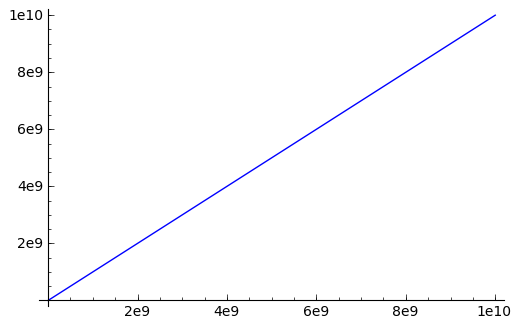
\includegraphics[height=4cm]{figures/x.png}}
	\hfill
	\subfloat[$10^x$]{\label{10hochx}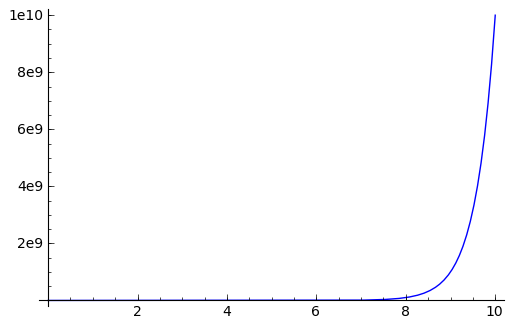
\includegraphics[height=4cm]{figures/10hochx.png}}
	\caption{Graph of the functions $x$ and $10^x$}
	\label{xund10hochx}
        \vskip +25pt 
\end{figure}


\subsubsection*{The function $\ln{x}$}
In comparison to that we consider the function $\ln{x}$. The left picture of figure \ref{lnxbis} on page \pageref{lnxbis} shows the graph with the domain of definition from $1$ to $100$. On the right picture the domain of definition was chosen between $1$ and $10^{10}$.\\
One can see that the values of the function $\ln{x}$ grow slowly compared to the growth of the function $x$. This is visualizd by the graph of both functions in one picture shown in figure \ref{xundlnxundxdurchlnx} on page \pageref{xundlnxundxdurchlnx}. In addition to that the graph of the function $\frac{x}{\ln{x}}$ was drawn in the same figure.

\begin{figure}[!htb]
	\centering
	\subfloat[ ]{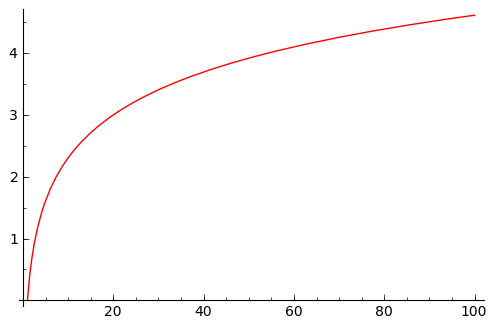
\includegraphics[height=4cm]{figures/lnxbis100.png}}
	\hfill
	\subfloat[ ]{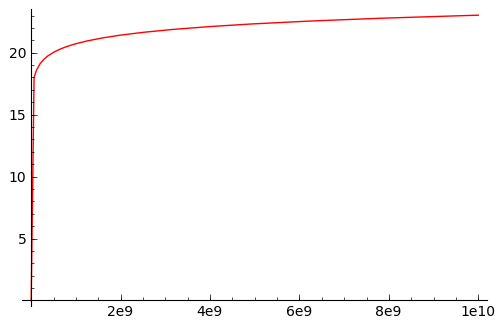
\includegraphics[height=4cm]{figures/lnxbis10hoch10.png}}
	\caption{Graph of the function $\ln{x}$ till $100$ and till $10^{10}$}
	\label{lnxbis}
        \vskip +25pt 
\end{figure}

\begin{figure}[!htb]
	\centering
	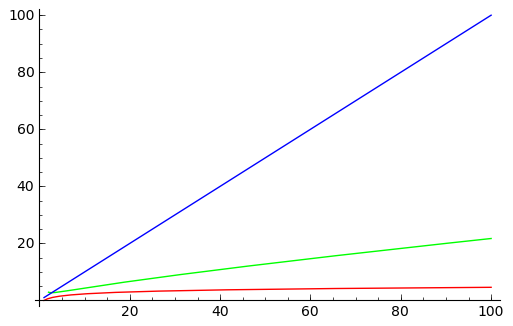
\includegraphics[height=4cm]{figures/xundlnxundxdurchlnx.png}
	\caption{The functions $x$ (blue), $\ln{x}$ (red)
                 and $\frac{x}{\ln{x}}$ (green)}
	\label{xundlnxundxdurchlnx}
        \vskip +25pt 
\end{figure}


\subsubsection*{The function $\frac{x}{\ln{x}}$}
The function $\frac{x}{\ln{x}}$ consists of the function $x$ as the numerator and the function $\ln{x}$ in the denominator, which, in comparison to $x$, increases very slowly. Compared to the number $x$ itself, the number of primes less or equal to $x$ is small. But still, $\frac{x}{\ln{x}}$ is an increasing function as you can see in figure \ref{xundlnxundxdurchlnx} on page \pageref{xundlnxundxdurchlnx}.


\subsubsection*{The number of primes in the different intervals}
To see how the number of primes in different intervals $[10^{x-1},10^{x}]$ behave, let's have a look on figure \ref{deltazehnxdurchlnxbis} on page \pageref{deltazehnxdurchlnxbis}. Here $\frac{10^{x}}{\ln{10^{x}}}$ and $\frac{10^{x}}{\ln{10^{x}}}-\frac{10^{x-1}}{\ln{10^{x-1}}}$ are visualized. The left chart shows the values for the exponent $x$ from $1$ to $5$ and the other one shows the values for $x$ from $1$ to $10$.\\
The blue bars represent the overall number of primes up to $10^x$. The red bars show how many primes lie in the interval $[10^{x-1},10^x]$, respectively. This makes clear, that the number of primes in intervals of higher exponents grows quite fast. 

\begin{figure}[!htb]
	\centering
	\subfloat[ ]{\label{deltazehnxdurchlnxbis5}
                     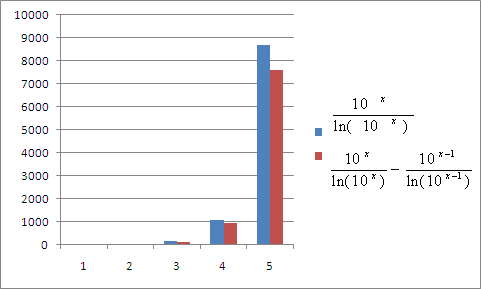
\includegraphics[height=4cm]{figures/deltazehnxdurchlnxbis5.png}}
	\hfill
	\subfloat[ ]{\label{deltazehnxdurchlnxbis10}
                     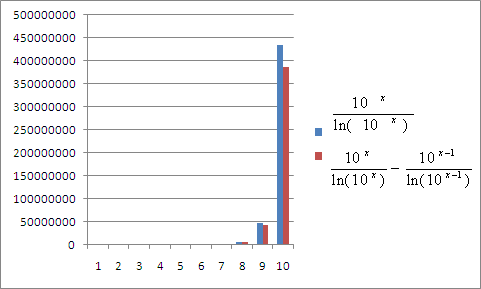
\includegraphics[height=4cm]{figures/deltazehnxdurchlnxbis10.png}}
	\caption{Numbers of primes in the interval $0$ to $10^x$ (blue) and in the intervall
                 $[10^{x-1},10^x]$ (red) for different exponents $x$.}
	\label{deltazehnxdurchlnxbis}
\end{figure}


A table containing the number of primes in some dedicated intervals can be found in
chapter \ref{s:primhfk} at page \pageref{s:primhfk}.




\begin{sagecode}
\begin{Verbatim}%
[fontsize=\footnotesize,fontshape=tt]

# Definition of function f(x)=x and plots for the domains from 0 to 10^10 and 0 to 100
sage: def f(x):return x
....:
sage: F=plot(f,(0,10^10))
sage: F.plot()

sage: F2=plot(f,(1,100))
sage: F2.plot()


# Definition of function g(x)=10^x and plots for the domain from 0 to 10
sage: def g(x): return 10^x
....:
sage: G=plot(g,(0,10))
sage: G.plot()


# Definition of function h(x)=log(x) and plots for the domains from 1 to 100 and 1 to 10^10
sage: def h(x): return log(x)
....:
sage: H=plot(h,(1,100),color="red")
sage: H.plot()

sage: H2=plot(h,(1,10^10),color="red")
sage: H2.plot()


# Definition of function k(x)=x/log(x) and plots for the domain from 2 to 100
sage: def k(x): return x/log(x)
....:
sage: K=plot(k,(2,100),color="green")
sage: K.plot()


# Plots of the functions f, k and h for the domain of definition up to 100
sage: F2+K+H


# Generation of the data for the bar charts ..........................
# Determination of the number of primes in the interval [1,10]
sage: pari(10).primepi()-pari(1).primepi()
4

# Determination of the number of primes in the interval [10^3,10^4]
sage: pari(10**4).primepi()-pari(10**3).primepi()
1061

# Determination of the number of primes in the interval [10^8,10^9]
sage: pari(10**9).primepi()-pari(10**8).primepi()
45086079

# (for 10^10: OverflowError: long int too large to convert)

\end{Verbatim}
\caption{Generation of the graphs of the three functions x, log(x) and x/log(x)}
\end{sagecode}



% ---------------------------------------------------------------------------
% ---------------------------------------------------------------------------
\clearpage
\newpage
\hypertarget{primes:_Appendix_Sage-Samples}{}
\section{Appendix: Examples using Sage}
% \section*{Appendix A: Examples using Sage}
% \addcontentsline{toc}{section}{Appendix A: Examples using Sage}
\label{primes:_Appendix_Sage-Samples}
\index{Sage!Code examples}
\index{Sage}

\noindent Below is Sage source code related to contents of the
chapter~\ref{Label_Kapitel_Primes} (``\nameref{Label_Kapitel_Primes}''). 


% ---------------------------------------------------------------------------
% \newpage
\subsection{Some basic functions about primes using Sage}
\index{Sage}

This part of the appendix contains Sage code, to perform some simple
computations about primes%
\footnote{See the Sage documentation about Elementary number theory
          \url{http://www.sagemath.org/doc/constructions/number_theory.html}.}.

\begin{sagecode}
\begin{Verbatim}%
[fontsize=\footnotesize,fontshape=tt]

# primes (general commands)
# The set of prime numbers
sage: P=Primes(); P
Set of all prime numbers: 2, 3, 5, 7, ...

# Returns the next prime number
sage: next_prime(5)
7

# Returns how many primes <=x are there
sage: pari(10).primepi()
4

# Returns the first x primes
sage: primes_first_n(5)
[2, 3, 5, 7, 11]

# Returns the primes in an interval
sage: list(primes(1,10))
[2, 3, 5, 7]

\end{Verbatim}
\caption{Some basic functions about primes}
\end{sagecode}



% ---------------------------------------------------------------------------
\newpage
\subsection{Check primality of integers generated by quadratic functions}
\index{Sage}

The following Sage code verifies the primality of integers generated
by the function $f(n) = n^2 - 9n + 61$.
The code defines a function called \verb!quadratic_prime_formula()!
that takes three arguments:
\begin{itemize}
\item \verb!start! --- An integer which is the lower bound for
  integers in the sequence $\texttt{start}, \texttt{start} + 1,
  \texttt{start} + 2, \dots, \texttt{end} - 1, \texttt{end}$.

\item \verb!end! --- An integer which is the upper bound for the
  integers in the sequence $\texttt{start}, \texttt{start} + 1,
  \texttt{start} + 2, \dots, \texttt{end} - 1, \texttt{end}$.

\item \verb!verbose! --- (default: \verb!True!) a flag to signify
  whether to print a message indicating the primality of an integer
  generated by $f(n)$.
\end{itemize}

\noindent A meaningful modification of this code is to use another function, of
which the primality of its function values should be checked.


\begin{sagecode}
\begin{Verbatim}%
[fontsize=\footnotesize,fontshape=tt]
def quadratic_prime_formula(start, end, verbose=True):
    print "N -- N^2 - 9*N + 61"
    P = 0 # the number of primes between start and end
    for n in xrange(start, end + 1):
        X = n^2 - 9*n + 61
        if is_prime(X):
            P += 1
            if verbose:
                 print str(n) + " -- " + str(X) + " is prime"
        else:
            if verbose:
                 print str(n) + " -- " + str(X) + " is NOT prime"
    print "Number of primes: " + str(P)
    print "Percentage of primes: " + str(float((P * 100) / (end - start + 1)))
\end{Verbatim}
\caption{Verify the primality of integers generated by a quadratic function}
\end{sagecode}

\vspace{12pt}
With the following function call we compute the values of $f(n) = n^2 - 9n + 61$ for
$n = 0, 1, 2, \dots, 50$ and verify the primality of the generated integers:

\begin{Verbatim}%
[fontsize=\footnotesize,fontshape=tt]
sage: quadratic_prime_formula(0, 50)
 N -- N^2 - 9*N + 61
0 -- 61 is prime
1 -- 53 is prime
2 -- 47 is prime
3 -- 43 is prime
4 -- 41 is prime
5 -- 41 is prime
6 -- 43 is prime
7 -- 47 is prime
8 -- 53 is prime
9 -- 61 is prime
10 -- 71 is prime
11 -- 83 is prime
12 -- 97 is prime
13 -- 113 is prime
14 -- 131 is prime
15 -- 151 is prime
16 -- 173 is prime
17 -- 197 is prime
18 -- 223 is prime
19 -- 251 is prime
20 -- 281 is prime
21 -- 313 is prime
22 -- 347 is prime
23 -- 383 is prime
24 -- 421 is prime
25 -- 461 is prime
26 -- 503 is prime
27 -- 547 is prime
28 -- 593 is prime
29 -- 641 is prime
30 -- 691 is prime
31 -- 743 is prime
32 -- 797 is prime
33 -- 853 is prime
34 -- 911 is prime
35 -- 971 is prime
36 -- 1033 is prime
37 -- 1097 is prime
38 -- 1163 is prime
39 -- 1231 is prime
40 -- 1301 is prime
41 -- 1373 is prime
42 -- 1447 is prime
43 -- 1523 is prime
44 -- 1601 is prime
45 -- 1681 is NOT prime
46 -- 1763 is NOT prime
47 -- 1847 is prime
48 -- 1933 is prime
49 -- 2021 is NOT prime
50 -- 2111 is prime
Number of primes: 48
Percentage of primes: 94.1176470588
\end{Verbatim}

\noindent The last two lines of the output contain a small statistics.
You can see that $f(n)$ generates
48 primes when $0 \leq n \leq 50$, which is approximately 94\% of the
values generated by $f(n)$.\\

For larger sequences, it is impractical to print all single messages indicating the
primality of integers. In the following Sage session, we count the
number of primes generated by $f(n)$ where $0 \leq n \leq 1000$ and
suppress primality messages.

\begin{Verbatim}%
[fontsize=\footnotesize,fontshape=tt]
sage: quadratic_prime_formula(0, 1000, False)
N -- N^2 - 9*N + 61
Number of primes: 584
Percentage of primes: 58.3416583417
\end{Verbatim}








% --------------------------------------------------------------------------
\newpage
\begin{thebibliography}{99999}
\addcontentsline{toc}{section}{Bibliography}


\bibitem[Aaronson2003]{pr:Aaronson2003} \index{Aaronson 2003}
    Scott Aaronson, \\
    {\em The Prime Facts: From Euclid to AKS}, \\
    \url{http://www.scottaaronson.com/writings/prime.pdf} \\
    After I had completed this article, I did come across the 
    fine paper by Scott Aaronson, which also offers
    a didactically very well-done introduction to this topic. It is 
    humorous and easy to read but at the same time precise and erudite.

% already defined in elementaryNumberTheory.inc -> 2 davor
\bibitem[Bartholome1996]{pr:2Bartholome1996}  \index{Bartholome 1996}
    A. Bartholom\'e, J. Rung, H. Kern, \\     
    {\em Zahlentheorie f\"ur Einsteiger}, Vieweg 1995, 2nd edition 1996.

\bibitem[Blum1999]{pr:Blum1999} \index{Blum 1999}   
    W. Blum, \\     
    {\em Die Grammatik der Logik}, dtv, 1999.

\bibitem[Bundschuh1998]{pr:Bundschuh1998} \index{Bundschuh 1998}
    Peter Bundschuh, \\
    {\em Einf\"uhrung in die Zahlentheorie}, Springer 1988, 4th edition 1998.

\bibitem[Crandell2001]{pr:Crandell2001} \index{Crandell 2001} \index{Pomerance 2001}
    Richard Crandell, Carl Pomerance, \\
    {\em Prime Numbers. A Computational Perspective}, Springer, 2001.

\bibitem[Doxiadis2000]{pr:Dioxadis2000}
    Apostolos Doxiadis, \\
    {\em Uncle Petros and the Goldbach's Conjecture}, \\
    Faber/Bloomsbury, 2000.

\bibitem[Graham1989]{pr:Graham1989} \index{Graham 1989}     
   R.E. Graham, D.E. Knuth, O. Patashnik, \\
   {\em Concrete Mathematics}, Addison-Wesley, 1989.

\bibitem[Klee1997]{pr:Klee1997} \index{Klee 1997}     
   V. Klee, S. Wagon, \\
   {\em Ungel\"oste Probleme in der Zahlentheorie und der Geometrie der 
   Ebene}, \\ Birkh\"auser Verlag, 1997.

\bibitem[Knuth1981]{pr:Knuth1981} \index{Knuth 1981}     
   Donald E. Knuth, \\ 
   {\em The Art of Computer Programming, vol 2: Seminumerical Algorithms}, \\
   Addison-Wesley, 1969, 2nd edition 1981.

\bibitem[Lorenz1993]{pr:Lorenz1993} \index{Lorenz 1993}     
   F. Lorenz, \\
   {\em Algebraische Zahlentheorie}, BI Wissenschaftsverlag, 1993.

\bibitem[Oppliger2005]{pr:Oppliger2005} \index{Oppliger 2005}
    Rolf Oppliger \\
    {\em Contemporary Cryptography},
    Artech House, 2005, \\
    \url{http://www.esecurity.ch/Books/cryptography.html}.

\bibitem[Padberg1996]{pr:Padberg1996} \index{Padberg 1996}     
   F. Padberg, \\
   {\em Elementare Zahlentheorie}, 
   Spektrum Akademischer Verlag 1988, 2nd edition 1996.

\bibitem[Pieper1983]{pr:Pieper1983} \index{Pieper 1983}     
   H. Pieper, \\
   {\em Zahlen aus Primzahlen}, 
   Verlag Harri Deutsch 1974, 3rd edition 1983.

\bibitem[Richstein1999]{pr:Richstein1999} \index{Richstein 1999}
    J. Richstein, \\
    {\em Verifying the Goldbach Conjecture up to $4*10^{14},$}
    Mathematics of Computation 70, 2001, p. 1745-1749). 

\bibitem[Scheid1994]{pr:Scheid1994} \index{Scheid 1994}
    Harald Scheid, \\ 
    {\em Zahlentheorie}, BI Wissenschaftsverlag, 2nd edition, 1994.

\bibitem[Schneier1996]{pr:Schneier1996p} \index{Schneier 1996}     
    Bruce Schneier, \\
    {\em Applied Cryptography, Protocols, Algorithms, and Source Code in C},\\
    Wiley and Sons, 2nd edition 1996.

\bibitem[Schroeder1999]{pr:Schroeder1999} \index{Schroeder 1999}
    M.R. Schroeder, \\
    {\em Number Theory in Science and Communication}, \\ 
    Springer 1984, 3rd edition 1997, Corrected Printing 1999.

\bibitem[Schwenk1996]{pr:Schwenk1996} \index{Schwenk 1996}     
    J. Schwenk \\
    {\em Conditional Access}, 
    in taschenbuch der telekom praxis 1996, \\
    Hrgb. B. Seiler, Verlag Schiele und Sch\"on, Berlin.

\bibitem[Shoup2005]{pr:Shoup2005} \index{Shoup 2005}
    Victor Shoup \\
    {\em A Computational Introduction to Number Theory and Algebra},\\
    Cambridge University Press, 2005, \\
    \url{http://shoup.net/ntb/}.

\bibitem[Tietze1973]{pr:Tietze1973} \index{Tietze 1973}     
    H. Tietze, \\
    {\em Gel\"oste und ungel\"oste mathematische Probleme}, \\
    Verlag C. H. Beck 1959, 6th edition 1973.

\end{thebibliography}


% --------------------------------------------------------------------------
\newpage
\section*{Web links} \addcontentsline{toc}{section}{Web links}

\begin{enumerate}
\item GIMPS (Great Internet Mersenne-Prime Search) 
      \index{Mersenne!prime number}  \index{GIMPS} \\
      www.mersenne.org is the home page of the GIMPS project, \\
      \url{http://www.mersenne.org/prime.htm}

\item The Proth Search Page with the Windows program by Yves Gallot \\
      \url{http://www.utm.edu/research/primes/programs/gallot/index.html}

\item Generalized Fermat Prime Search \\
      \url{http://primes.utm.edu/top20/page.php?id=12}

\item Distributed Search for Fermat Number Divisors \\
      \url{http://www.fermatsearch.org/}

\item At the University of Tennessee you will find extensive research
      results about prime numbers. \\
      \url{http://www.utm.edu/}

\item The best overview about prime numbers is offered from my point of view 
      by ~``The Prime Pages'' from professor Chris Caldwell.
      \index{Caldwell Chris} \\
      \url{http://www.utm.edu/research/primes}

\item Descriptions e.g.\ about prime number tests \\
      \url{http://www.utm.edu/research/primes/mersenne.shtml} \\
      \url{http://www.utm.edu/research/primes/prove/index.html}

\item Showing the $n$-th prime number \\
      \url{http://www.utm.edu/research/primes/notes/by_year.html}

\item The supercomputer manufacturer SGI Cray Research not only 
      employed brilliant mathematicians but also used the prime 
      number tests as benchmarks for its machines. \\
      \url{http://www.isthe.com/chongo/tech/math/prime/prime_press.html}
	 
\item The Cunningham Project, \index{Cunningham project}\\ 
      \url{http://www.cerias.purdue.edu/homes/ssw/cun/}

\item \url{http://www.eff.org/awards/coop}

% \item \url{http://www.informatik.tu-darmstadt.de/TI/LiDIA/}

\item \url{http://www.math.Princeton.EDU/~arbooker/nthprime.html}
% {\tt http://www.math.Princeton.EDU/\~{}arbooker/nthprime.html }

\item Goldbach conjecture verification project von Tom�s Oliveira e Silva,
      \index{Goldbach project}\\ 
      \url{http://www.ieeta.pt/~tos/goldbach.html}

\item \url{http://www.mathematik.ch/mathematiker/goedel.html}

\end{enumerate}



\vskip +10 pt
% --------------------------------------------------------------------------
\section*{Acknowledgments}
\addcontentsline{toc}{section}{Acknowledgments}

I would like to take this opportunity to thank Mr.\ Henrik Koy and Mr.\ Roger
Oyono for their very constructive proof-reading of the first versions
of this article.



% Local Variables:
% TeX-master: "../script-en.tex"
% End:
